\documentclass{report}
\usepackage{fullpage}
\usepackage{graphicx}
\usepackage{pdfpages}
\usepackage{amsmath}
\usepackage{float}
\graphicspath{{figures/}}
\title{Design of An Innovative, Highly Maneuverable, Stealthy Unmanned Underwater Vehicle with ISR Capabilities }
\setlength{\parindent}{4em}
\author{Brian Martin\\ Ben Saletta\\Andrew Blancarte\\ Ketton James\\Abraham Paucar}
\date{\today}
\renewcommand{\chaptername}{Phase}
\renewcommand{\bibname}{References}
\begin{document}
\maketitle
\tableofcontents
\listoffigures
\newpage
\section{Introduction}
Newton’s third law of motion states that when two bodies interact, there are equal and opposite reactions that occur. Propulsion works on this principle and it is what allows an object to move forward. In terms of marine vehicles, a propulsion system (typically a propeller) accelerates water (the working fluid) which produces a thrust force on the propeller and body that moves the vehicle forward. In the world of marine propulsion, bladed propellers have dominated since the creation of paddle wheel by the US Navy in the 1840s.\par
\subsection{Traditional Issues}
Today, bladed propellers are by far the most common means of propelling water crafts, whether above or below the surface. While bladed propellers are effective, relatively inexpensive to manufacture, and available in a wide variety of sizes and geometries, they also exhibit numerous inefficiencies and disadvantages.  Among these are that they create flow instabilities (buffeting), cavitate easily (leading to accelerated degradation as a result of surface pitting), produce a significant amount of noise (mainly as a result of cavitation), must be made of heavy, metallic materials (in order to mitigate the effects of cavitation damage), and are exposed to foreign object damage (which can lead to fouling which is detrimental to its primary function). These shortcomings can become greatly exaggerated when bladed propellers are used for fully submerged vehicles; this is especially true for applications in which stealth is key, such as in military submarines, special operator deployment craft, and unmanned undersea drones such as remotely operated vehicles (ROVs), unmanned underwater vehicles (UUVs), and autonomous underwater vehicles (AUVs).  \par
The objectives for this project are to produce the UV to have fluid/smooth maneuvering, be capable of higher speeds (relative to other UVs), require little to no human interaction, and to boast a great deal of stealth (with respect to thermal, magnetic, and flow signatures, noise, cavitation, and ability to be inconspicuous).\par
The idea of underwater exploration is not new, however, stealthy UVs that can overcome the shortcomings inherent to traditional propellers and designed ISR missions is not a fully developed industry.\par
\subsection{Competition}
The idea of underwater exploration is not new, however, stealthy UVs that can overcome the shortcomings inherent to traditional propellers and designed ISR missions is not a fully developed industry. \par
A commercial company called OpenROV sells small tethered, battery powered ROV that is market as an underwater exploration vehicle for everyone. It uses three propellers as its propulsion system which achieves a maximum speed of 2 knots, and maximum operational depth of 246 feet. Although its size and price are impressive, it does not improve or acknowledge the aforementioned issues produced by the propellers and therefore does not meet the mission and operational objectives set out.\par
However, completion exists in the form of a 5 foot, 100 pound, US Navy developed, underwater drone codenamed GhostSwimmer. The US Navy, in collaboration with Boston Engineering, had developed and tested swarms of this new UUV which uses an innovative, biomimetic oscillating tail fin to produce thrust, eliminating the use of a traditional propeller altogether. Visually, GhostSwimmer looks likes and replicates the movements of actual tuna and by doing so can achieve an operational maximum speed of 3 knots and operational depth of 300 feet. It is highly maneuverable and versatile, able operate using battery power and remotely by a 500 foot tether. According the release from the Navy on December 11, 2014, Ghostswimmer “gathered data on tides, currents, wakes and weather conditions -- the sort of oceanographic information commonly gathered by meterologists and submariners for use in finding -- or concealing -- subs.” This UV meets both the mission and operational objectives set out and, in some areas, surpasses them. The fact that GhostSwimmer exists simply means that the work and research Team UV has done is warranted. \par
\subsection{Our Solution}
As previously demonstrated, the underwater vehicle market has been expanding in recent years to include a number of new vehicles and technologies; however, many of these new solutions fall victim to the same inefficiencies that underwater vehicles have been plagued by for years, especially within the context of stealth.  The solution that we put forth in the coming pages aims to revolutionize the way that naval ISR is performed by taking more special operators out of the field to make their jobs easier and less dangerous.\par
In order to define how our solution will stray from the traditional underwater vehicle, two sets of parameters were defined.  The first set is termed the "Mission Objectives" and provides a set of guidelines for the project.  The second set is termed the "Operational \& Design Objectives" and represents the specific performance goals for the final project; unlike the Mission Objectives, the Operational \& Design Objectives are subject to change throughout the evolution of the project. \par
\subsection{Mission Objectives}
These Mission Objectives are our top priority goals for this project and represent the mandatory deliverables for this project; this is to say that every decision for the project was first evaluated against these Mission Objectives so as to ensure that none of these objectives were violated, as said violation would constitute a breach of mission and thus a failure of objectives.  These objectives were developed prior to the start of Phase I in April 2014 and are listed below for reference.
\begin{enumerate}
\item Fluid/smooth maneuvering
\item Higher speeds
\item Stealth
\subitem Thermal Signature
\subitem Magnetic Signature
\subitem Noise
\subitem Flow Signature
\subitem Cavitation
\subitem Inconspicuous
\item Little or no human interaction required
\end{enumerate} 
*These objectives were set out in the initial concept stage of this project and must be carried through to the final design/testing phases.  Violation/endangerment/jeopardizing of these mission objectives is equivalent to a failure of the mission; as such, these mission objectives should be upheld throughout the project period and must be repeatedly referenced for compliance.\par
\subsection{Operational \& Design Objectives}
The Operational \& Design Objectives essentially set in place the practical definite parameters of the design (whereas Mission Objectives refer to the more global, superficial characteristics of the vehicle as a whole) and were originally laid out at the beginning of Phase I.  These objectives are listed below for reference:
\begin{itemize}
\item Depth range of ~100-200 ft
\item Speed of ~ 5 knots
\item Size limited to approximately that of a scuba tank
\item Weight which aims to increase thrust-to-weight ratio, but reduce the amount of positive buoyancy that the buoyancy control systems must overcome; the weight might possibly be used to induce neutral buoyancy at a prescribed depth
\item Operational times of ~ 1 hour at full power
\item Maximization of internal space for stowage of the sensor suite
\item Eases of storage and transportation/portability
\item Ease of maintenance/reduction in required maintenance
\end{itemize}
These Operational \& Design Objectives were more comprehensively assessed at the end of the Summer 2014 time period as a means of altering the objectives to a refined state consistent with the progress/success of Phase I \& II, while keeping in mind the timeline and scope of work for Phase III.  The changes to the Operational \& Design Objectives that reflect the updated performance goals heading into Phase III are as follows and correspond to the italicized items within the initial Operational \& Design Objectives list as noted above:
\begin{enumerate}
\item Reduced operational depth range to match the depth capabilities of commercially available buoyancy control solutions as found in preliminary component identification/costing research to a ~33 ft (1 atm) test depth capability and ~66 ft maximum operational (buoyancy control limiting) depth of ~66 ft (2 atm).
\item Reduced speed goals to correspond to the balance between vane shell propulsor optimization, manufacturing challenges (tolerance limitations), and body drag (as effected by the battle between streamlining and manufacturing limitations).
\end{enumerate}
\subsection{Brief Project Overview}
The timeline for this project is split into three phases over a 14 month period; these phases (along with truncated descriptions of the phases) are as follows.\par
Phase I (ME 325/L\_Spring 2014): As the introductory phase of the project, this phase (spanning 36 days from April 2014 to May 2014) focused on the development of the propulsion system demonstrator for the project.  Based off of the findings regarding the plausibility and efficiency of Phase I, the developed propulsion system demonstrator would be directly integrated into the full vehicle as the propulsor, adapted towards the vehicle propulsor, or scrapped in favor of a different propulsor for the vehicle.\par
Phase II (Summer Research/Testing\_Summer 2014): This follow-up phase began the same day that Phase I ended (in May 2014) and ran until the day that Phase III began (in September 2014).  The focus of this phase consisted of three main goals: future vehicle concept development, literary research, and experimental testing.  With regards to future vehicle concept development, the team spent a great deal of time conceiving, visualizing, and documenting ideas for what the final vehicle would look like and what kind of subsystems it would be composed of; this sub-focus of Phase II continued into the early stages of Phase III.  The majority sub-focus of Phase II was the literary research, which spanned very many topics in engineering (many of which were extremely advanced, high-level topics), as will be discussed later.  The final subset of Phase II, experimental testing, consisted of both propulsion system demonstrator testing and small-scale testing aimed at gaining further insight into the physics associated with the demonstrator’s flow mechanics and into the requisite considerations that would be associated with future subsystems.\par
Phase III (Senior Project\_Fall 2014, Winter 2015): This phase began the same day as Phase II ended (in September 2014) and will officially end at the end of the Winter 2015 quarter (in March 2015), but will unofficially continue until all aspects of the project are completed (projected June 2015).  The official time span of this phase will cover the development of the full vehicle, the building of said vehicle, and the testing of the vehicle.  The unofficial appended time span will cover research conferences, presentations, further development, and further testing of the vehicle, with the unofficial end of the phase coming with the last deliverable for the project (at the time of writing, this would be the senior project symposium/possible show case or the California State University Student Research Conference – CSUSRC, both of which will be discussed in the section of conferences/talks).  Specific subsystems for further development in this phase consist of:
\begin{itemize}
\item Propulsion System
\item Maneuverability Systems
\subitem Control Surfaces
\subitem Control Electrical Systems
\subitem Control Programming
\item Buoyancy Control Systems
\subitem Buoyancy Control (Mechanical) Systems
\subitem Buoyancy Control Electrical Systems
\subitem Buoyancy Control Programming
\item Body
\subitem Streamlining
\subitem Subsystem Housing
\subitem Structural Support System
\item Navigation
\subitem Electrical Systems
\subitem Programming
\item Sensor Suite
\subitem Navigation Components \& Programming
\subitem ISR Components \& Programming
\item	Graphical User Interface (GUI)
\end{itemize}
Phase III will require greater incorporation of subjects/theories such as mechanical design, electromechanical systems, materials selection, fluid mechanics, heat transfer, acoustics, computer programming, and many more. More information about the specific phases, Phase III goals/challenges/etc., and scope of work, please see the appended Senior Project Primer Package.
\chapter{Propulsor Development, SHEILA-D}
\section{Overview}
SHEILA-D stands for Subaquatic Hydrodynamicaly propelled Explorer Implementation Los Angeles - Demonstrator. The driving force behind the development of this unmanned underwater vehicle is the innovative propulsion system. This system was the foundation of the first phase of development, a proof of concept for this screw based propulsion system. As this phase was a deliverable for a Machine Design Class there is a detailed overview of this phase included in appendix A. 
\section{Constraints}
As this initial design was part of a class project there were many constraints that came along with it. The primary constraint was time. The project was completed, from design to testing, in 35 days to meet the deadline imposed by the academic calender. There were also significant cost constraints because this phase was funded completely out of the personal funds of the members involved. The constraints eliminated several custom manufacturing techniques due to extensive lead times and costs. This led to the final construction consisting mainly of parts shaped from hardware store components.
\section{Design}
The initial design phase took the first 5 days in which the foundational fluid mechanics, the drive train and power calculations were completed in these days. Further redesign was included in with the manufacturing process when the aforementioned constraints restricted the construction of the device as designed.
\subsection{Fluids Calculations}
The fluids calculations were an important part of the initial design because of the roll they played in moving the device through the water. To complete these calculations the device was broken into two sections. First the cylinder holding the screw and second the cone used to accelerate the fluid. For the cylinder an assumption was made that a constant force would be imparted to the fluid along the surface of the screw blades. This constant force would act on the fluid mass between the vanes therefore, assuming a constant density, the vanes would provide a constant acceleration along this section. With a known length of the cylinder and this calculated acceleration the speed of the fluid exiting the cylinder was calculated. Conservation of momentum was then applied to the fluid as it passed through the final cone and nozzle giving the final thrust force of the propulsion system. These calculations were plugged into an Excel spreadsheet and various geometries were iterated through to find the optimal configuration. A more detailed walk through of the fluids analysis is included in appendix A.
\subsection{Drive Train}
The fluids calculations provided a value for the required torque and angular velocity. The drive train was designed to meet both of these criterion. The major difficulty with the drive train in this design was transmitting the torque from the motors to the external shell. To solve this problem and provide sufficient torque two motors were fitted with gearboxes then mated to the sun gear in a planetary gear set that transmitted the torque out to the rotating cylinder as seen in Figure 1.1. The planetary gear system was 3D printed to minimize cost and manufacturing time.
\begin{figure}[h]
\centering
\includegraphics[width=15cm]{"Section View"}
\caption{Drive Train Design Section View}
\end{figure}
\subsection{Power Supply}
These motors required a significant amount of current at a constant 12 volts. These requirements went into the power design calculations and searches for sufficient batteries. A single 12 volt lithium battery was selected due to its high current discharge, compact form, and high capacity characteristics. The design of the power supply was integrated into the design of the drive train due to the important relationship between the easily available motors and batteries for a reasonable operational time. The power supply had to fit between the two motors and is shown as a black box in Figure 1.1.
\section{Construction}
The construction of this device was completed in a very short time span using commercial off the shelf components. This involved PVC pipes of various diameters, cutting and thermoforming sheets of acrylic, and fastening components with traditional fasteners as well as epoxy. As the construction proceeded difficulties were discovered and the design was adjusted to compensate for these problems. One of the major difficulties was the manufacture of the helix screw. This was solved by thermoforming cut acrylic then filling gaps created in the vanes with waterproof tape. Other adjustments and quick fixes were applied through out the process. The construction was a challenge to complete within the time frame at an acceptably low cost.  
\section{Testing}
Once construction was completed the device needed to be tested to confirm that the propulsion system did indeed propel the device through the water. To do the testing properly the vehicle was taken to the Puddingstone reservoir at dawn and ran along the deck of a boat dock. It took a few tests to get the device operational and, while the vehicle could not be set off on its own at this stage, it pumped a significant amount of water though the body and out the cone and nozzle assembly. Many things were learned about the design during the testing session and made note of for future design. The major lessons were that the assumptions that were made in the fluid calculations were wrong and that without control surfaces the vehicle would reach an equilibrium rotation state where the outermost cylinder would rotate and counter the rotation of the center cylinder. 
\chapter{Summer Research and Testing}
During the summer of 2014 the group members of Team UV did not entirely part ways for three months. The group decided that it would be in the best interest of the group and design itself to meet twice a month where each member would give presentation on standard material along with research they have found during the two week period between meetings. These meetings started in June of 2014 and ended when the 2014 Fall period started, September 2014.  Each of the meetings held were roughly five to seven hours long. The format of the presentations were standardized however each member provided their own research and information. Presentation format can be found in appendix B. In the summer of 2014 Team UV spent roughly 240 hours as a group towards the senior project itself. That number includes research done outside of the meeting along with the meetings themselves. The PowerPoint presentations contained three sections.
\section{Open Mind}
The group was given a situation/problem that has or could happen in the world we live in today and each member had to give insight or propose a solution to the problem/situation. Each member were asked to provide their solution along with reasoning  as to why their solution would be efficient. Since Team UV are composed of mechanical engineering undergraduates, the solutions based on the prompts were required to use some aspect of engineering. For example, one open mind prompt addressed the issue that many people in developing countries lack the access to power. The group was asked if they were tasked with developing an inexpensive “do it yourself” power generation system for use in a 3rd world country, what kind of engineering considerations might you take into account. The idea behind the open mind prompt was to keep the group members mind engaged during the break and keep that engineering mentality sparked. Also, this prompt was to have the members think outside the box and to aid in developing creative/innovative ideas for use in the senior project design.
\section{Well-Read}
Members were asked to look into articles/publications and present something they found to be interesting, innovative, advancements, etc. The articles were not limited to strictly the engineering field however it was recommended.  Articles presented from the group ranged from next generation wind turbines to theory behind the process of suction eating of fish. The idea of the well-read was to give insight to the group of remarkable advancements in science and technology throughout the world.
\section{Presentation}
The presentation was an open ended section which allowed for each member to present some research they did during the two week period between meetings. The research was required to aid in the design of the senior project in areas such as theory, analysis, design, controls, manufacturing, and/or testing. Research in CLT propellers, computational fluid dynamics, Arduino coding, wake turbulence, underwater designs and coatings, power management, component selection for marine research, smart ducts, submarine design/research, and many others. 
\section{Summer Research Summaries}
\subsection{Shark Skin}
\begin{figure}[h]
\centering
\includegraphics[width=5cm]{"Shark Skin"}
\caption{Close up of Shark Skin}
\end{figure}
Sharks move very efficiently thanks to the characteristics of their skin.  Anything but smooth, shark skin has individual scales, called dermal denticles, with narrow passages that reduce friction drag and accelerate the flow along its length.  These scales also flex and realign to reduce biofouling which can negatively affect flow over the body.

\subsection{Vantablack}
\begin{figure}[h]
\centering
\includegraphics[width=5cm]{"Vantablack"}
\caption{Vantablack on Aluminum Substrate}
\end{figure}
Surrey NanoSystems has engineered a new super-black material called Vantablack.  This material composed of “Vertically Aligned Carbon Nanotube Arrays” absorbs 99.965\% of incident light.  Photons are allowed into the material and are then blocked and trapped from leaving.  This material is already in high demand for space and stealth applications. 

\subsection{Cephalopod Skin}
\begin{figure}[h]
\centering
\includegraphics[width=5cm]{"Cephalopod Skin"}
\caption{Cephalopod Skin}
\end{figure}
Two teams of researchers from Rice University and MIT were tasked with developing material which could replicate the camouflaging abilities of cephalopods.  The class of mollusks which include squid, possess skin that can manipulate its own color and texture.  Rice University engineering a rigid aluminum nanorod display panel which displays an intense color spectrum.  MIT, on the other hand, created a flexible display that can change color and texture but with limited color spectrum.

\subsection{Waterproofing Sensors}
\begin{figure}[h]
\centering
\includegraphics[width=4cm]{"Potting"}
\includegraphics[width=6cm]{"Conformal Coating"}
\caption{Potting and Conformal Coating}
\end{figure}
Using sensors underwater with a strict budget takes a bit of creativity.  Two popular methods used by hobbyists and professionals alike are: Potting and Conformal Coating.  Potting is the method of filling an electronic assembly with a solid or gelatinous compound such as a thermosetting plastic or silicone.  This blocks water and increases shock resistance.  Conformal Coating offers the same benefits of potting but is lighter and non-permanent which allows for reworking.
\subsection{Arduino}
\begin{figure}[h]
\centering
\includegraphics[width=5cm]{"Arduino UNO"}
\caption{Arduino Uno Microprocessor}
\end{figure}
Microprocessing is made accessible to all thanks to companies like Arduino.  Boards housing everything from input and output terminals to a microprocessor can link the electrical world to the physical world.  Users start out controlling the lighting sequencing of LED’s to eventually controlling more advanced mechanical systems.  Topics presented to the team include LED control, reading data from sensors, and ways to expand the factory limitations of Arduino boards.  
\subsection{CFD and Python}
Computational Fluid Dynamics, CFD, is a powerful tool for the analysis of fluid behavior. The computational techniques used to break down the navier-stokes equations have applications that stretch beyond the realm of fluid dynamics and allow the modeling of many non linear mathematical phenomena within a computational environment. This presentation was an introduction to the ideas behind CFD and the way that an analysis could be written using the Python coding language.
\subsection{Physical Understanding of Fluids Equations and their Application to CFD}
To apply any of the fundamental fluids equations to a device a physical understanding of the meaning behind the mathematics is crucial. This presentation addressed four different ways to address a fluids problem. First analysing a stationary control volume and applying conservation of mass equations to the borders. Secondly selecting a moving control volume of fixed mass and applying conservation of momentum equations to the borders. Thirdly selecting an infinitely small particle and analyzing the fluid that passes through it. Or finally selecting an infinitely small particle and analyzing its path through the fluid. This allows for the analysis of any problem from a variety of different perspectives.
\subsection{Optimal Design of an Archimedes screw}
As the device that we are manufacturing depends upon a screw similar to the original archimedes screw it was important that we analyze the methods used to optimize the design of one of these screws.\cite{Rorres00} This introduced the idea of breaking a design down into dimensionless variables that dictated the ratio of the size of components and reduced the amount of unknown variables. These dimensionless numbers were then varied and efficiencies were calculated providing the final, most efficient design ratios.
\subsection{Tom's Effect}
Fish are covered with mucus primarily to cover wounds and promote healing, however this mucus also causes Tom’s Effect. This is when a high molecular weight polymer is released into a fluid stream it makes the fluid remain laminar for longer because the polymers line up with the streamlines in the fluid. This requires the fluid to use more energy to break the streamlines and become turbulent. With fish this allows them to travel through the water with significantly less drag than they otherwise would have had to overcome. The could be applied to any underwater vessel to provide increased fuel efficiency and stealth.
\subsection{WHOI Acoustic Modem}
 Underwater communications have been a long standing challenge because radio waves attenuate rapidly in water. A possible method for communication between several underwater vehicles or even between a vehicle and its home base is an acoustic modem. These work by emitting modulated sound waves that carry data through the water. Due to the high speed of sound through water these methods of communication become practical. 
\subsection{CLT Propellers}
\begin{figure}[h]
\centering
\includegraphics[width=5cm]{"CLT"}
\caption{Contacted and Loaded Tip Propellers}
\end{figure}
Fundamentally the goal of the Contracted and Loaded Tip (CLT) propeller is to improve open water efficiency.  This means that the tip on the propeller reduces the velocities of water entering the propeller disk which, in turn, reduces the hydrodynamic pitch angle.  This reduction of hydrodynamic pitch angle and induced velocities results in many advantages.  To list a few, CLT propellers achieve higher top speeds, greater thrust, smaller optimum propeller diameter, better maneuverability, inhibits cavitation and tip vortices (resulting in less noise, less vibrations, lower pressure pulses, and lower area ratio
\subsection{Smart Duct}
\begin{figure}[h]
\centering
\includegraphics[width=5cm]{"Smart Duct"}
\caption{Thrust Vectoring Smart Duct}
\end{figure}
A Smart Duct is a deformable shroud that changes the direction of flow of the propeller wash to provide a direct steering force to the vehicle.The duct itself is an electrically actuated structure that is covered by a flexible hydrodynamically smooth sheathing whose primary movers are a set of high strength Nickel-Titanium SMA actuator cables.  Shape memory alloys (SMA) make this deformable Smart Duct a reality. Testing has proven flow turning angles of up to 15 degrees at thrust levels of operational submarines is possible with this technology.  These results may directly affect the design of future marine vehicles by reducing (and possibly eliminating) the use of control surfaces for maneuvering.
\subsection{Vortex Generators}
\begin{figure}[h]
\centering
\includegraphics[width=5cm]{"Vortex Generators"}
\caption{Vortex Generators on the Wing of a Fighter Jet}
\end{figure}
For relatively blunt objects like a sphere or wing on a plane the overall drag decreases when the boundary layer becomes turbulent because turbulent flow allows the boundary layer to follow the surface closer which decreases the overall wake region.  The larger this wake region is the more you see chaotic flow separation and adverse pressure gradients that can be catastrophic on aircraft because the flow separation can cause them to stall.Vortex generators can be found on the wings of aircraft and even on some high performance cars.  With vortex generators there is an exchange between high energy momentum and lower energy momentum by tripping laminar flow into turbulent which allows the boundary layer to remain attached over a greater length of the wing chord or car profile which results in a thinner wake region and smaller adverse pressure gradient on the rear of the object which lowers the pressure drag.  This allows for many benefits like lowering the stall speed, improving stability and control during maneuvering, and decreasing the turning radius.
\subsection{Wanda II}
\begin{figure}[h]
\centering
\includegraphics[width=5cm]{"Wanda II"}
\caption{Wrasse-inspired Agile, Near-shore, Deformable-fin Automation}
\end{figure}
Researchers have turned to nature for inspiration trying to model a UUV that uses flapping fins to maneuver through difficult underwater environments.  Many fish species use articulation of the pectoral fins to produce appropriate forces and moments propel themselves through the water and to react to dynamic changes in flow, physical obstacles, and wave forces near the shore. A four-fin UUV named WANDA-II (Wrasse-inspired Agile Near-shore Deformable-fin Automaton) is the 2nd generation of this alternative propulsion UUV. These fins are capable of producing thrust vectors in multiple directions through changes in curvature and stroke angle. All this is in the attempt to replicate the high level of controllability that fish species have near shore and in shallow water environments. A four-fin UUV could be deployed in a variety of missions including harbor monitoring and protection, hull inspection, and covert shallow water operations. 
\subsection{Control Surface Basics}
\begin{figure}[h]
\centering
\includegraphics[width=5cm]{"Pitch Roll Yaw"}
\caption{Representation of Euler Angles}
\end{figure}
Control Surfaces are moveable surfaces on wings that allow for maneuverability for both air and marine vehicles. Typically when control surfaces deflect they change the trailing edge of the wing which in turn changes the angle of attack. Angle of attack is the angle of between the wing chord (leading edge to trailing edge) to the Relative Airflow or free air flow (RAF). The amount of lift a wing produces is more a function of the angle of attack rather than the shape of the airfoil (cross section of the wing).The primary control surfaces on an airplane are ailerons (which controls roll/pitch), elevators (which controls pitch), and the rudder (which controls yaw).
\subsection{Materials and Stealth}

“…five major underwater vehicle requirements.  The two key issues are technical feasibility and stealth.  The third important issue is survivability.  Fourth, and equally important is the need to successfully deliver a payload.  And finally, all of these attributes regardless of importance, must be considered within a framework of cost.” (Submarine Technology for the 21st Century).\par
\begin{figure}[h]
\centering
\includegraphics[width=5cm]{"Submarine Stealth"}
\caption{Sonar Detection of a Submarine}
\cite{sonar}
\end{figure}
Research was done into submarine hull materials and what we could learn from them for our project within the framework of parameters such as weight/speed, strength/depth capability, stiffness, corrosion resistance, magnetic signature, machinability/formability, fatigue resistance, thermal properties, electrical properties, and acoustic properties.  Research was conducted into steel, titanium, aluminum, composites (Carbon Fiber-, Titanium-, and Glass Fiber-Reinforced Polymers), and general polymers.\par
\par Stealth was investigated with regards to passive control (active control was not looked into owing to the impracticality with regards to the scope/scale of our project).  Passive control research centered firstly on the effect of polymeric bodies and polymer secretion on the hydrodynamic boundary layer, skin friction, wake field, general turbulence, vortices, and hydrodynamic noise generation.  The next direction for passive control was towards acoustic stealth via the use of anechoic materials (with sublayers for absorbing sonar waves, damping and decoupling of internal signal waves, and transmission layers for areas with intentional signal emission/transmission) and machinery “raft” beds (for vibration and noise damping), including attenuation ranges, elastomeric viscoelastic mechanical models, porosity effects (on attenuation, damping, and chemical stability), the correlation of relaxation modulus with temperature, signal frequency, and thermal transitions, and chemical stability (hydrolytic stability and water absorption).
\subsection{Funding}
Research was conducting with regards to sources of project financial support.  Options looked into included National Science Foundation (NSF) and Department of Defense (DoD) grants, innovation competition awards, (financial, material, product, and service) sponsorships (and the possible development of a sponsorship brochure) and donations, and online crowdsourcing.  The final decision was to use crowdsourcing for the majority of the fundraising and to look for sponsors and donors whenever possible.  Specific companies further researched for sponsorship, donation, or discount included Proto Labs, Rapid Machining, Quick Parts, Solid Concepts, and the Cal Poly Pomona Southern California Engineering Technologists Association (SCETA).\par
Websites looked into for hosting the crowdsourcing campaign included KickStarter, Indiegogo, RocketHub, and GoFundMe.  Aspects considered included campaign type [Flexible (keep what you raise) vs. Fixed (all or nothing)], timeline, campaign durations, processing/collection timelines and fees, donor rewards, website demographics (aimed at technical or artistic people), website traffic, and connectivity with social media.\par
At this time, the team also created social media accounts with Facebook, Instagram, and Twitter in order to help spread awareness of both the fundraising campaign and the website (which was created through WordPress.com after consideration and research into the same basic considerations as for the fundraising campaign, with the addition of website cost, domain ownership, and customization considerations).
\subsection{Testing}
Research was also conducted into both industry standard marine vehicle testing (mostly the use of tow tanks and the specific parameters often focused on with industry testing, i.e. the Admiralty Coefficient) and testing that we could perform. \par
\begin{figure}[h]
\centering
\includegraphics[width=5cm]{"Test Tank"}
\caption{Underside of a Boat in a Tow Tank}
\cite{TowTank}
\end{figure}
The first future test highlighted for our project included powered movement testing with stabilizing surfaces (for cancelling out torque transfer and rotation transmitted to the outer body) and a distributed weight belt (for inducing neutral buoyancy) with the parameters of interest of water speed, thrust, and flow field visualization.  Other test ideas consisted of battery run time tests, sealing tests, and small scale concept tests (i.e. using a cut open 2L bottle, cone to fit into the bottle, and swirling motion to determine the most efficient exit flow type through measuring drain time and waterproofing small DC motors and connecting them to vane shells of various geometries inside submerged tubes).
\subsection{Thrust Augmentation}
Research was conducted into Zone I (hull and pre-shaft inlet sections), Zone 2 (fluid working section), and Zone III (outlet section) thrust augmentation devices, their implementation, and how they influence propulsive efficiency, flow separation, turbulence, propulsor swirl (pre-swirl and post-swirl) (and thus flow equalization), cross flow minimization (and thus bilge vortices), effective thrust, shaft vibrations, wake field magnitude and distribution, open water efficiency, energy recovery, propeller hub vortices, conversion of rotational kinetic energy to directional flow, hydrodynamic lift, and lift-drag ratio.  Devices researched include:
\begin{itemize}
\item Zone I: Wake equalizing ducts, asymmetric sterns, Grothues spoilers, stern tunnels, semi- or partial ducts, reaction fins, Mitsui Integrated Ducted Propulsion Units, and Hitachi Zosen Nozzles.
\item Zone II: Increased diameter-low RPM propulsors, Grim Vane Wheels, propellers with end-plates, CLT propulsors, and propeller cone fins.
\item Zone III: Rudder-Bulb fin systems and additional thrusting fins.
\end{itemize}
\begin{figure}[h]
\centering
\includegraphics[width=5cm]{"Thrust Augmentation"}
\caption{Thrust Augmentation on the Hull of a Ship}
\cite{Grotheus}
\end{figure}
\indent Research was also conducted into the effect of combination of devices with the conclusion that most combinations were not possible due to one device removing the regime utilized by the other, while a select few combinations led to good benefits.
\subsection{Owl Stealth}
\begin{figure}[h]
\centering
\includegraphics[width=8cm]{"Owl Stealth"}
\caption{Wing Features on an Owl that Provide Stealthy Flight}
\cite{OwlWing}
\end{figure}
Research was conducted into the mechanisms by which owls derive their acoustic stealth, with the goal of better understanding the turbulent eddies and their amplification/scattering from the trailing edges of wings (natural or man-made) and how biomimicry might be able to change the way our control surfaces might affect our stealth (acoustic or flow signature).  Research centered on the profiles, material properties (most importantly stiffness), geometry, and surface roughness of the leading edge, mid-wing section, and trailing edge.\par
It was determined that the trailing edge is the dominant noise source on wings and that owl wing stealth was mainly the result of use of leading and trailing edge tubercles and flexible, porous trailing edge material.  Tubercles were to be a future feature of our vehicle's control surfaces, time permitting.
\subsection{Submarine Hydrostatics}
\begin{figure}[h]
\centering
\includegraphics[width=8cm]{"Submarine Hydrostatics"}
\caption{Center of Buoyancy and Center of Mass of a Submarine}
\cite{hydrostatics}
\end{figure}
Research was conducted into ship and submarine hydrostatics in the surfaced, diving/surfacing, and submerged states.  Key factors considered included state of buoyancy, reserve of buoyancy, trim, configuration and use of main ballast tanks (internal and external), free flood spaces, margin ballasts, variable ballasts, superstructures, flexible bag ballasts with flotation collars, freeboard, and a pressure hull.\par
\indent Methodologies for buoyancy calculation were researched heavily for both intact and damaged vessel states, surface (static), surfacing/diving (transition), and submerged (static) states, conditions of flotation, and disturbance response for small and large values of sway, yaw, surge, heave, and (the most complex case) heel/roll.\par
\indent Some specific takeaways included the final decision with regards to buoyancy control system and flood/vent hole design (i.e. location and use of a grill if requiring a large hole in order to disrupt noise, vibration, and drag caused by the flood/vent hole(s)).
\subsection{Submarine Design Process}
\begin{figure}[h]
\centering
\includegraphics[width=5cm]{"Submarine Design"}
\caption{Design Considerations for Underwater Vehicles}
\cite{design}
\end{figure}
Research was conducted into the submarine design process as presented in Concepts in Submarine Design, 2s (Burhcer).  This design process is shown below, with the accelerated modifications for our time-sensitive project shown in red.\par
Note: Bolded text in the following paragraphs highlights the applicability to our project. Specific topics focused on included  role designation \textbf{(ISR)} [and subsequent subrole \textbf{(perform ISR in a covert manner within a variety of environments while retaining high stealth, maneuverability, elevated speeds, and sufficient battery life)]}, development of operational requirements \textbf{(specifics of speed, maneuverability, battery life, stealth characteristics, etc. requirements)}, concept studies (with key parameters of size, cost, payload, performance), feasibility studies (and system material requirements) \textbf{(development of weight, space, and power budgets for various sub-systems in design)}, \textit{design for build} (detailed systems, subsystems, arrangements, configurations, specifications, etc. \textbf{(management of previously developed budgetary allocations with deliverables relating to structures, arrangements, hydrodynamics, subsystems, hydrostatics (both surface and submerged), etc.)}, and production design \textbf{(final vehicle design)}.
\subsection{Buoyancy Control}
A research article contained information related to buoyancy control of a semiautonomous underwater vehicle and design orientation. The orientation of the design determined what the application of the vehicle. For example, if the design were to be horizontal resembling a manta ray, its use would be for towing and exploration at lower depths. However, due to this orientation it has a higher chance of getting stuck in densely populated sea vegetation or between underwater rocks. If the orientation were to be vertical, resembling a fish, its use would be for a remote controlled mode and towing as well. The vertical orientation makes it easier to maneuver in densely populated sea vegetation. The buoyancy control mechanism contained two compressed air tanks connected to two separate balloons. The air would be released into the balloon when the vehicle needed to raise and the air would be released the vehicle needed to be lowered.
\subsection{Underwater Coatings}
Cathodic protection is used in a vary of underwater applications. Cathodic Protection (CP) is a technique used to control the corrosion of a metal surface by making it the cathode of an electrochemical cell. A simple method of protection connects the metal to be protected to a more easily corroded "sacrificial metal" to act as the anode. The sacrificial metal then corrodes instead of the protected metal. The sacrificial metal that has been corroded provides a protective surface to prevent the base material from being corroded. Alocit by the A\&E group is an coating that is used for underwater applications. It is one of three coatings that meet the specs of the US Army Corps of Engineers.
\subsection{Currents}
\begin{figure}[h]
\centering
\includegraphics[width=5cm]{"Currents"}
\caption{Currents and Overall Fluid Transport}
\end{figure}
Currents are broken down into two types, surface and deep water. Deep water currents usually occur more than 400 meter (~1300 feet) under the surface of the water. The water movements are caused by differences in water density known as Thermohaline circulation. Deep water currents are much slower than surface currents but they move much more water due to water density increase deeper in the sea. Surface currents are due to the Coriolis Effect. The Coriolis Effect occurs due to the rotation of the earth, the circulating air is deflected resulting in curved paths. The wind’s curved path drags on the water’s surface, causing it to move in the direction the wind is blowing. The Ekman Spiral is a consequence of the Coriolis Effect.
\section{TeamUV.org}
Establishing TeamUV.org was the obvious next step after a Summer filled with professional growth and academic exploration.  Not only was the website about the current progress of the team’s senior project but also about inspiring interest in STEM and facilitating monetary support.  Topics covered range from fluid dynamics, robotics, and biomimicry to shining light on what engineering is and how it impacts the world.  Inspired by websites often visited by Team UV members, posts were uploaded various times throughout the week to keep followers intrigued without feeling overwhelmed.  Well Reads, Presentations, and Open Minds were set to be posted on Tuesdays, Thursdays, and Sundays, respectively.  Each post was written by a team member according to a set schedule set for months in advance.  A list of website postings can be found in Appendix .  Team UV also made sure that the website was linked with companion Facebook, Twitter, Instagram, and GoFundMe accounts.\par
\indent Team UV.org went live on July 31, 2014 with a welcome post about the site, the project, and ways to help the team’s fundraising campain.  The site instantly created buzz pulling in 122 views and 38 visitors the first month.  After gaining a steady following from all around the world including 87 countries, TeamUV.org achieved a best month of 670 views and 518 unsubscribed visitors in January 2015.  To date, the site has gained a steady, recurring base of 84 subscribed followers that actively visit and participate in leaving comments for the team.\par
\indent Aside from weekly posts, visitors to the site can also find team member biographies giving background about personal interests, academic experiences, and professional work.  Those looking to sponsor the team’s efforts with donations or equipment are also able to give directly on the site, follow a  link to the Team UV GoFundMe site, or contact the them directly.  

\section{Summer Testing}
Along with delving into Summer research pertaining to many aspects of engineering design, Team UV also performed a couple of tests.  Another trip to Sailboat Cove was made to test the benefits of attaching control surfaces to Sheila-D.  Spring Quarter testing resulted in the formation of a free exit jet but minimal displacement of the vehicle.  Due to stacking inefficiencies with material availability, available manufacturing methods, and unaddressed torque transfer issues, Sheila-D was in need of support.  Scrap square pieces of aluminum flashing were roughly attached to the sides of the propulsor which controlled the overturning moments caused by torque transfer in the device.  This resulted in linear travel along the dock, verifying the projects potential.\par
Testing the importance of the exit cone was also performed during the summer session.  2-liter soda bottles were modified to resemble the flow through Sheila-D.  Water was passed through the model’s nozzle. with and without an exit cone, and discharge times were recorded.  The use of the exit cone was verified by the faster exit times of the cone-equipped soda bottle.  Tests were also performed as to the effects of pre-swirl into the nozzle caused by the vane shell.  Tests using modified soda bottles showed promising results as the water look to discharge out the nozzle faster with pre-swirl but were eventually ruled inconclusive.  Controlling the swirl of the exiting water was difficult to accomplish giving the tests poor repeatability.\\
\chapter{Final Prototype Design and Manufacture, DORY}
\section{Lessons Learned}
Even though SHEILA-D was able to provide thrust through the use of the unique propulsion system there were factors that attributed to the inefficiencies of SHIELA-D. For example, SHEILA-D was funded entirely from the group members themselves and was under a deadline of eight weeks to do analysis, design, manufacture, and testing. Contacting vendors to manufacture customized parts where tolerances were very critical was found to be very expensive.  Therefore components bought for SHEILA-D were products that could be obtained from readily available sources with little to know lead time from local vendors such as Home Depot or bought online from vendors such as McMaster Carr. SHEILA-D was not designed from components that could be bought locally or online which led to the team adjusting many components ultimately leading to a greater manufacturing timeframe. The main inefficiency during phase I was the high amount of friction that occurred in the system. The main component of the propulsion was experiencing a high amount of friction which caused the first round of testing to fail. The team took these experiences into high consideration when designing the phase III device.\par
The revised goal resulting from the experiences of phase I was to minimize friction in the system and develop an entire underwater vehicle that overcomes the shortcomings of a traditional propeller system. The new phase III device would have an entirely remote operation which eliminates the need to tether the device. The device would perform its mission in obtaining information, surveillance, and reconnaissance (ISR). In order to achieve this goal several new components were added to the phase III device to ensure enough information is received. To ensure sufficient maneuverability three control surfaces powered by servo motors were added to the design. The phase III device was made to be neutrally buoyant therefore a piston ballast tank was added to control the depth of the vehicle. The vehicle’s rotational power is going to be provided by only one motor instead of 2 motors to give more room for additional components. The biggest addition to phase III was the use of a graphical user interface (GUI). The GUI is where the user would read all of the information received by the vehicle once it has returned from its mission. The GUI has four separate components that display specific information. One box will display a video of the route the vehicle took. This will be achieved by placing a camera at the face of the vehicle that saves the data onto a SD card. The second box displays information on the vehicles speed, displacement, and orientation. An accelerometer will be placed inside the vehicle in order gain this information. The third box shows the orientation of the vehicle. Orientation data is taken from the accelerometer and the model will update the orientation to show how the vehicle was oriented at a specific time. The fourth box contains a map that plots the route of the vehicle. When the vehicle ends its mission the map will display the route it took. The electronics will be powered by batteries and functionality to be provided by the use of an Arduino. The GUI was to be done using the program, Processing.\par
\section{Subsystem Decomposition}
\subsection{Propulsor}
\subsubsection{Control Volumes}
In order to perform our internal fluids analysis on the propulsor with the goal of optimizing the vane shell, we had to treat the problem as a basic fluid mechanics problem and start with the same foundational elements of all fluid mechanics problems; we had to define some control volumes.\par
Before jumping right into defining our control volumes, we had to identify the parameters of interest to us; of these, we highlighted four main parameters that were to be treated as unknowns:
\begin{enumerate}
\item Inlet velocity at the front of the propulsor $v_1$
\item Pressure at the end of the vane shell and prior to the nozzle $P_2$
\item Exit velocity at the rear of the nozzle $v_3$
\item Thrust force produced by the vehicle $F_T$
\end{enumerate}
Additionally, these values would be evaluated at three main state points:
\begin{itemize}
\item The free stream inlet region ahead of the propulsor $(1)$
\item The interface between the back of the vane shell and the start of the nozzle/cone$(2)$
\item The exit region immediately behind the nozzle $(3)$
\end{itemize}
To properly solve for these four unknowns, we needed four equations and thus we developed four control volumes $(A, B, C, D)$, each with a distinct equation associated with it as will be shown below.  Once we had these four equations developed, the plan was to use an iterative programming technique to solve the four equations for the four unknowns, thus yielding the parameters necessary for finding the basic performance characteristics associated with the propulsor.  This will be discussed in greater detail in the programming section of the report that follows.\par
As will be seen below, the basic types of equations utilized in the analysis consisted of the conservation of energy and the conservation momentum; conservation of mass was not utilized as it did not yield any helpful information with regards to the problem solving process.\par
\begin{equation}
\frac{P_i}{\gamma}+\frac{v_i^2}{2g}+h_{L_{i-f}}=\frac{P_f}{\gamma}+\frac{v_f^2}{2g}+h_{s_{i-f}}
\end{equation}
\begin{equation}
\Sigma F=P_iA_i+\dot{m}v_i+P_fA_f-\dot{m}v_f-F_T+F_D=ma
\end{equation}
\paragraph{Control Volume A}
For control volume $A$, the energy equation was adopted, with the unknowns of $v_1$ and $P_2$.
\begin{figure}[H]
\centering
\includegraphics{"Ctrl Volume A"}
\caption{Schematic of Control Volume A}
\end{figure}
\begin{figure}[H]
\centering
\includegraphics{"Eqn A"}
\caption{Simplified Energy Equation for Control Volume A}
\end{figure}
As can be seen, the inlet pressure term was set equal to zero, as this was taken to be gage pressure since it is simply the free-stream hydrostatic field pressure.  The two elevation terms also cancel, because even if the propulsor was stood up vertically, the change in elevation would only be one to three feet (this length had yet to be determined), which would be negligible; additionally, the vast majority of the time, the vehicle would be travelling at roughly zero angle of attack (and therefore would not have a change in elevation from front to back of the propulsor).\par
This leaves a few terms remaining; $g$ is simply the gravitational acceleration (32.2 $\frac{ft}{s^2}$), $\gamma$ is simply the specific weight of the fluid (water; 62.4 $\frac{lb}{ft^3}$), $v_1$ is the inlet velocity (an unknown, as defined earlier), $P_2$ is the pressure at the end of the vane shell (another unknown, as defined earlier), $v_2$ is the velocity at the end of the vane shell, $h_{L_{1-2}}$ is the energy loss term from front to back of the vane shell, and $h_{s_{1-2}}$ is the shaft input energy term from front to back of the vane shell.\par
In order to reduce this equation further to the original two unknown values we wished to solve for, we had to come up with equations for the $v_2$, $h_{L_{1-2}}$, and $h_{s_{1-2}}$ terms.\par
Using the fact that $v_2$ represents the maximum speed our vane shell could get the fluid moving without slip, we defined the maximum vane shell axial fluid speed to be equal to the angular velocity times the effective screw pitch associated with the vane shell, which is a function of the average radius (average between the base radius, or outside radius of the cylinder onto which the vanes attach and the maximum radius, or the radius to the tips of the vanes) and the angle of twist of the vanes:
\begin{equation}
v_2=\omega P;p=\frac{2\pi r_{avg}}{\tan(\theta)}
\end{equation}
The next term is the head loss term along the length of the vane shell ($h_{L_{1-2}}$); this term would normally include both major (due to friction) and minor losses (due to components), but since there is not any major bends/corners/etc., the minor losses were neglecting, reducing the head loss term to that of purely major loss.
\begin{equation}
h_{L_{1-2}}=f\frac{L}{D_h}\frac{v^2}{2g}
\end{equation}
The velocity ($v$) used above would be taken as the average between the free stream velocity ($v_1$, an unknown) and the maximum/end of vane shell velocity ($v_2$) and thus would require iteration in the program.  The length of the vane shell ($L$) would be assumed in the iteration at different values in order to determine the desired unknown values over a range of lengths.  The hydraulic diameter ($D_h$) would be determined for each set of iterations on the basis of assumed vane shell geometry (just like the length), through the formula:
\begin{equation}
D_h=\frac{4A}{P}
\end{equation}
where $A$ is the area of the flow (determined by finding the sum of all inter-vane flow areas, as restrained by vanes on either side of the flow, the rotating cylinder on the bottom of the flow, and the stationary body cylinder on the top of the flow).  Lastly, the friction factor ($f$) was determined as the Darcy-Weisbach friction factor through the use of the Swamee-Jain approximation of the Colebrokk-White equation:
\begin{equation}
f=\left\{\begin{array}{ll}
\frac{64}{Re}&:Re\leq2000~~Laminar\\
.25[\log(\frac{\epsilon}{3.7D_h}+\frac{5.74}{Re^{.9}})]^{-2} &:Re>2000~~Turbulent\\
\end{array}
\right.
\end{equation}
\begin{equation}
Re=\frac{v_{avg}D_h}{\nu}
\end{equation}
where $\eta$ is the material roughness,$Re$ is the Reynolds number as defined in equation 3.7, and $\nu$ is the kinematic viscosity of the fluid.
Lastly, the shaft head ($h_{s_{1-2}}$) was taken as:
\begin{equation}
h_{s_{1-2}}=\frac{T\omega}{\gamma Q}
\end{equation}
where $\omega$ is the rotational speed (as defined earlier), $\gamma$ is the specific weight (as defined earlier), $Q$ is the volumetric flow rate (the product of the average velocity and the flow area, as both defined earlier), and $T$ is the torque.  Torque was defined as a fluid torque through its relation to the rotational speed of the screw-like vane shell and the twist of the path of water (more details about this may be found in the appended original Phase I report calculations, appendix A):
\begin{equation}
T=\frac{(r_avg\omega)^2}{2g}\gamma A \cos(\Phi)(r_avg)
\end{equation}
With all of these equations developed, it becomes apparent that the original energy equation (after substitution of assumed geometry and iterated angular velocities) has been reduced to two unknowns ($v_1$ and $P_2$), albeit in a highly intertwined fashion.
\paragraph{Control Volume B}\par
For control volume $B$, the energy equation was again adopted, this time with the unknowns of $P_2$ and $v_3$.
\begin{figure}[H]
\centering
\includegraphics{"Control Volume B"}
\caption{Schematic of Control Volume B}
\end{figure}
\begin{figure}[H]
\centering
\includegraphics{"Eqn B"}
\caption{Simplified Energy Equation for Control Volume B}
\end{figure}
Once again, elevations cancel, one pressure (this time the exit pressure) interfaces with the hydrostatic pressure field and is thus set to zero gage pressure, and this time the shaft input energy term is set to zero because we are now beyond the vane shell and only have stationary components.  $P_2$ (an unknown) is defined the same as before, $v_2$ is the maximum/end of vane shell velocity (as defined earlier), and $v_3$ (also an unknown) is the free jet exit velocity, as defined earlier.  This just leaves the head loss term, which unlike before now contains both major (due to friction and calculated the exact same way as before, except between points 2 \& 3, rather than 1 \& 2) and minor losses (due to components).  The minor losses were modeled through use of the following general minor loss equation:
\begin{equation}
h_{L_{2-3}(minor)}=K\frac{v_{avg}^2}{2g}
\end{equation}
where $K$ is the component loss coefficient, which in this case was taken conservatively as the worst case non-reentrant scenario entrance loss coefficient ($K=0.5$), although our situation would never come near this scenario.
\begin{figure}[H]
\centering
\includegraphics[width=8cm]{"Nozzel Minor Losses"}
\caption{K values for Minor Losses due to Diameter Change}
\end{figure}
With all of these equations developed, it becomes apparent that the original energy equation (after substitution of assumed geometry and iterated angular velocities) has been reduced to two unknowns ($v_3$ and $P_2$), albeit in a highly intertwined fashion.
\paragraph{Control Volume C}\par
For control volume $C$, the momentum equation was adopted, with the unknowns of $P_2$, $v_3$, and the thrust force $F_T$.
\begin{figure}[H]
\centering
\includegraphics{"Control Volume C"}
\caption{Schematic of Control Volume C}
\end{figure}
\begin{figure}[H]
\centering
\includegraphics{"Eqn C"}
\caption{Simplified Energy Equation for Control Volume C}
\end{figure}
$P_3$ is once again set to zero gage as it is the hydrostatic field pressure, drag force ($F_D$) is assumed zero for the small nozzle section, and acceleration ($a$) is taken to be zero due to the assumption that steady state velocity (no acceleration) has been reached.  $P_2$, $v_2$, and $v_3$ are defined as before and the thrust force ($F_T$) is one of the desired unknowns.  $A_2$ is the area of the annular flow region between the circular nozzle and the circular pressure hull/start of cone (not pictured).  This just leaves the mass flow rate ($\dot{m}$), which is the product of the average velocity from point 2 to 3, the density of the fluid (water), and the effective flow area as previously discussed.\par
Once again, with all of these equations developed, it becomes apparent that the original momentum equation (after substitution of assumed geometry and iterated angular velocities) has been reduced to three unknowns ($v_3$, $P_2$, and $F_T$).
\paragraph{Control Volume D}
For control volume D, the momentum equation was adopted, with the unknowns of $v_1$, $v_3$, and the thrust force $F_T$.
\begin{figure}[H]
\centering
\includegraphics{"Control Volume D"}
\caption{Schematic of Control Volume D}
\end{figure}
\begin{figure}[H]
\centering
\includegraphics{"Eqn D"}
\caption{Simplified Energy Equation for Control Volume D}
\end{figure}
Just as before, $P_1$ and $P_3$ are both taken to be zero gage due to their interfacing with the hydrostatic field pressure and the acceleration is set to zero due to assumed steady state operation; also as seen previously, $v_1$, $v_3$, and $F_T$ are all desired unknowns and mass flow rate is calculated the same as before, with the average velocity being taken between points 1 and 3.  The only new term being introduced here is the drag force ($F_D$).\par
The drag force is calculated with the classic algebraic form of the drag force equation:
\begin{equation}
F_D=0.5\rho C_D v^2 A
\end{equation}
where $\rho$ is the fluid (water) density, $v$ is the average velocity between points 1 and 3, $A$ is the reference area (in this case taken as the outermost circular cross-sectional area of the body cylinder), and $C_D$ is the drag coefficient, which has been taken conservatively to be $1.2$.\par
One last time, with all of these equations developed, it becomes apparent that the original momentum equation (after substitution of assumed geometry) has been reduced to three unknowns ($v_1$, $v_3$, and $F_T$).
\paragraph{Integration of Control Volumes}
With all of these control volumes and the associated equations, it can be seen that we have developed four equations (the ones boxed in red in the previous sections) as a function of four desired unknowns ($v_1$, $P_2$, $v_3$, $F_T$).  As can be seen the system of four equations is statically determinant with the right assumptions made, but is nonlinear in nature and highly inter-dependent, requiring a very complex computer program to be written in order to integrate the four equations together to solve for the desired unknowns, as will be discussed in the next section.  A summary of the desired unknowns for each control volume is provided below.
\begin{enumerate}
\item Control Volume A (Energy Equation from 1 to 2): $v_1$ and $P_2$
\item Control Volume B (Energy Equation from 2 to 3): $P_2$ and $V_3$
\item Control Volume C (Momentum Equation from 2 to 3): $P_2$,$v_3$, and $F_T$
\item Control Volume D (Momentum Equation from 1 to 3): $v_1$, $v_3$ and $F_T$
\end{enumerate}

\subsubsection{MatLab Code}
The mathematical model rendered through the above control volume analysis still contained many unknowns. With the above equations the relationship between these unknowns could be determined, however finding the optimal value of each of the 5 geometrical dimensions and the one dynamic variable would have required exhaustive iterations and guess work. To facilitate the design process and ensure optimal design a program was written in the MatLab coding environment that would cycle through ranges of each of these variables, creating every possible combination of designs and rank them on an efficiency. This would allow for the most efficient design to be selected.\par
The majority of the variables in question described the geometry of the propulsor. To reduce the complexity of the design some variable were designated before the program began. The length of the nozzle was fixed to 5 inches, providing a reference size so that the most efficient design would still have a reasonable package size. The number of vanes was set to 5, in previous iterations of the program a value of 5 vanes commonly populated the highest efficiency and therefore it was set, freeing up processing time for more volatile variables. The outer radius, inner radius, length, angle of the vane helix, and nozzle radius were allowed to vary. Each variable had to have a range to vary within because without a finite range the program would loop infinitely. The maximum outer radius was set to 5 inches, the minimum inner radius was set to 2 inch, length ranged between 18 and 26 inches, the vane angle varied between 42 and 48 degrees, the minimum nozzle radius was .75 inches.\par
%INSERT TABLE WITH INITIAL RANGES AND VARIABLES%
\begin{table}[h]
\begin{center}
\begin{tabular}{l|c|c}
Variable&Minimum Value& Maximum Value\\
\hline
Outer Radius, $r_o$&& 5 in\\
Inner Radius, $r_i$&2 in&\\
Length, $L$ &18 in&26 in\\
Vane Angle, $\theta$&42$^{\circ}$&48$^{\circ}$\\
Nozzle Radius $r_n$&.75 in&\\
Rotational Velocity $\omega$ & 220 RPM & 320 RPM\\
\hline
\end{tabular}
\end{center}
\caption{Iteration Ranges for Design Variables}
\end{table}
The dynamics of the system also had to be coded into the program. The angular velocity was the only parameter allowed to vary from a low speed of 50 rad/sec to 200 rad/sec. A pump efficiency of .75 was used to account for losses in energy transfer from the vanes to the fluid itself, the surface roughness of PVC was used because it most accurately modeled the material we anticipated the vane shell to be made of. A drag coefficient of 1.2 was used as a conservative estimate, the real drag will be much less because the outer surface will be streamlined.\par
\begin{table}[h]
\begin{center}
\begin{tabular}{l|c|c}
Variable&Value& Source\\
\hline
Acceleration due to Gravity, $g$&32.2$\frac{ft}{s^2}$&\cite{munson}\\
Specific Weight, $\gamma$&62.4 $\frac{lb}{ft^3}$&\cite{munson}\\
Kinematic Viscosity, $\nu$&12.1$*10^{-6}\frac{ft^2}{s}$&\cite{munson}\\
Surface Roughness, $\epsilon$&0.0015mm&\cite{munson}\\
\hline 
\end{tabular}
\end{center}
\caption{Material Constants for Design}
\end{table}
 %INSERT TABLE OF VARIABLES WITH REFERENCES%
Not every variable needed a range to vary within because certain relationships were established. This allowed for more accurate results while still minimizing the amount of processing time. The minimum outer radius was limited to be at least .25in greater than the inner radius to allow for a practical vane height. The nozzle maximum value was limited so that the exit area would never exceed the area of the annular region between the inner cylinder and the outer cylinder. This was done to ensure that the the nozzle would be converging and provide increased thrust rather than the diverging nozzle that would slow the fluid and reduce the overall thrust.  \par
With these relationships and ranges established the order of the nested loops needed to be established. The loops were ordered so that the more depended on the variable being changed the farther out of the nest it was placed. This led to the following order: angular velocity, inner radius, outer radius, nozzle radius, length, then vane angle. By nesting the loops in this order all of the relationships between the different range limits could be satisfied and once in the center of the loops one complete set of design variables was established.\par
In the center of the nested loops two finite difference loops were used to assist in the solving of the mathematical models derived from the control volume analysis. The first finite difference loop calculated the friction factor used to find the losses along the length of the vane shell. The second finite difference loop was used to find the friction factor for the losses through the nozzle. These losses were used with the established design variables to find the overall thrust, the pressure at the end of the vane shell, the speed of the device at steady state, and the speed of the free jet leaving the end of the nozzle.\par
These results from the fluid analysis were used to determine the efficiency of the device. The energy added to the fluid increased the velocity up to the end of the vane cylinder. A 100\% efficient device would move at the speed of the fluid at this point. Essentially a fully efficient device would accelerate until it could no longer add energy to the fluid. This means that the efficiency of the device could be calculated by taking the steady state speed of the device and dividing it by the steady state speed of the fluid after the vane shell. $\eta=\frac{V_1}{V_2}$. These calculations were done for all the possible combinations of design parameters within the given ranges resulting in thousands of possible designs each with their own efficiency.\par
\subsubsection{Excel Narrowing of Results}
All of the designs were exported in a comma separated value format to be manipulated in Excel. First all efficiency values less than or equal to zero were removed as poor designs, then each variable was graphed with respect to efficiency. Due to the cyclic nature of the analysis data was plotted as clusters around certain values. Using these plots the clusters of data with low efficiency could be eliminated. Certain geometrical values were limited by realistic manufacturing constraints. This means that very small clearances between the inner radius and outer radius were removed along with  excessively small nozzle radi. By narrowing these results in this fashion final design values were arrived upon with a resulting efficiency of between 77.8\% and 80.7\% for a range of angular velocities. The final geometry was.
%INSERT TABLE WITH FINAL GEOMETRY%
\begin{table}[h]
\begin{center}
\begin{tabular}{l|c}
Variable& Value\\
\hline
Outer Radius, $r_o$&4.45in\\
Inner Radius, $r_i$&3.2in\\
Length, $L$ &19.6in\\
Vane Angle, $\theta$&48$^{\circ}$\\
Nozzle Radius $r_n$&1.218 in\\
\hline
\end{tabular}
\end{center}
\caption{Final Geometry for the Propulsor Design}
\end{table}
\subsubsection{CFD}
Computational Fluid Dynamics, or CFD, is a numerical technique for solving the Navier-Stokes equations and mathematical modeling a fluid’s behavior under specific circumstances. The Navier-Stokes equations do not have an explicit analytical solution but they are commonly used to model ideal cases where certain simplifying assumptions can be made, such as neglecting viscosity or compressibility. Before these computational techniques complicated fluid analysis was performed using experimentation with models. As designs involved more complicated geometries and fluid reactions such as with a super sonic jet iterative modeling experiments became excessively expensive in both time and money.  This, along with the evolution of computers, led to the development of these computational techniques.
To understand further look at the Navier-Stokes Equaton:
\begin{equation}
\frac{\partial{\vec{V}}}{\partial{t}}+(\vec{V}\cdot\nabla)\vec{V}=\frac{-\nabla P}{\rho}+\nu\nabla^2\vec{V} 
\end{equation}
The $(\vec V\cdot\nabla)\vec V$ adds non-linearity to the equation while $\nu\nabla^2\vec{V}$ makes the system second order. These added complexities make the analytical solution of the equations practically impossible.For a numerical solution to be achieved first a numerical grid must be set up. Each node in the grid represents a position in space with an added dimension of time. This is because the dynamics of the fluid depend on the surrounding fluids as well as its position at the previous time. To understand the full dynamics of the fluid in question the whole grid must be solved for every point in time. Computational techniques can only handle addition, subtraction, multiplication, and division, no calculus. This means the equation needs to be transformed into a numerically solvable form. For this the Taylor Series expansion can be used.\par
The generic Taylor Series is as follows:
\begin{equation}
u(x)=\sum_{n=0}^{\infty}\frac{f^{(n)}(x_i)}{n!}(x-x_i)^n
\end{equation}
Solving the Taylor series for the $f^{(n)}$ term allows for the numerical solving of the differentials in the Navier Stokes equations. If the Taylor Series is solved on the previously discussed numerical grid for a one dimensional flow the following relationship is achieved:
\begin{equation}
\frac{\partial{u}}{\partial{x}}\bigg|_i=\frac{u_{i+1}-u_{i}}{x_{i+1}-x_i}-\frac{x_{x+1}-x_i}{2!}\frac{\partial^2u}{\partial x^2}\bigg|_i-\cdots
\end{equation}
If the grid spacing,$(x_{i+1}-x_i)$, is close enough the equation can be truncated with an error of $\frac{x_{x+1}-x_i}{2!}\frac{\partial^2u}{\partial x^2}\big|_i$. This allows for a simply algebraic solution to a partial derivative and is the function that gives CFD its power.\par
These solutions still need set boundary conditions, such as velocity or pressure, the properties of the fluid, such as density and viscosity, as well as the properties of the design being tested, most significantly the geometry. Once these characteristics are imputed the program iterates through each point in space, solving the Navier-Stokes equations with the appropriate Taylor substitutions, then it moves to the next point in time and solves again until the designated amount of time has passed. The inputed conditions give the program a place to begin and therefor are an important consideration in the overall solution.\par
With a good understanding of the basics of CFD the student version of AutoCAD CFD was used along with SolidWorks FlowAnalysis to find the solutions for our specific geometry. To prove our concept with CFD the design was steped through and analysis was done with each added flow component.
\paragraph{Analysis of the Vane Shell}
Traditional propellors have no ducting around them and this is one of the major things this design improves. As a starting point CFD analysis was done on just the vane shell.
\begin{figure}[H]
\centering
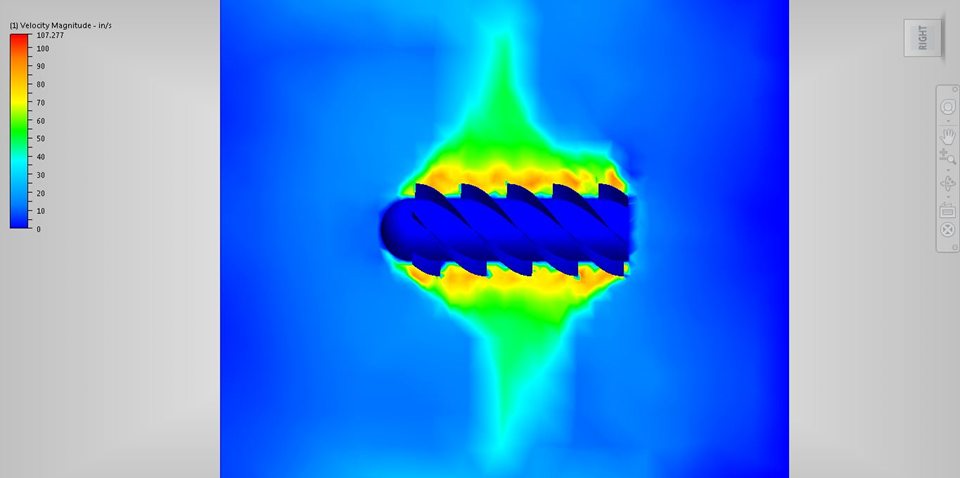
\includegraphics[width=12cm]{CFDvs}
\caption{CFD Analysis of the Vane Shell}
\end{figure}
This image shows that much of the energy added to the fluid by the propulsion system is lost by accelerating the fluid radially.
\paragraph{Analysis of the Vane Shell and Body}
Analysis was run again with the addition of a bounding duct around the vane shell to constrain the fluid so that all acceleration of the fluid with be along the length of the propulsor. 
\begin{figure}[H]
\centering
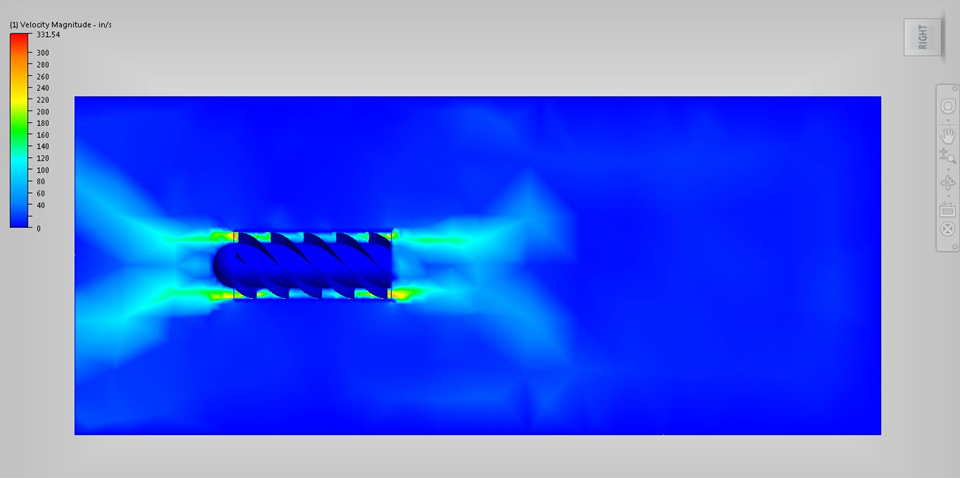
\includegraphics[width=12cm]{CFDvsb}
\caption{CFD Analysis of the Vane Shell with the Body}
\end{figure}
As this figure shows the fluid is now directed along the length of the device, however at the tail end there is a triangular section of flow recirculation and the flow is not fully constrained and deviates at the rear. This reduces the amount of thrust produces as well as increasing amount of drag acting on the device.
\paragraph{Analysis of the Vane Shell, Body and Nozzle}
The addition of a nozzle at the end of the device constrains the flow and increases the velocity of the fluid leaving the device increasing the amount of thrust produced due to the conservation of momentum.
\begin{figure}[H]
\centering
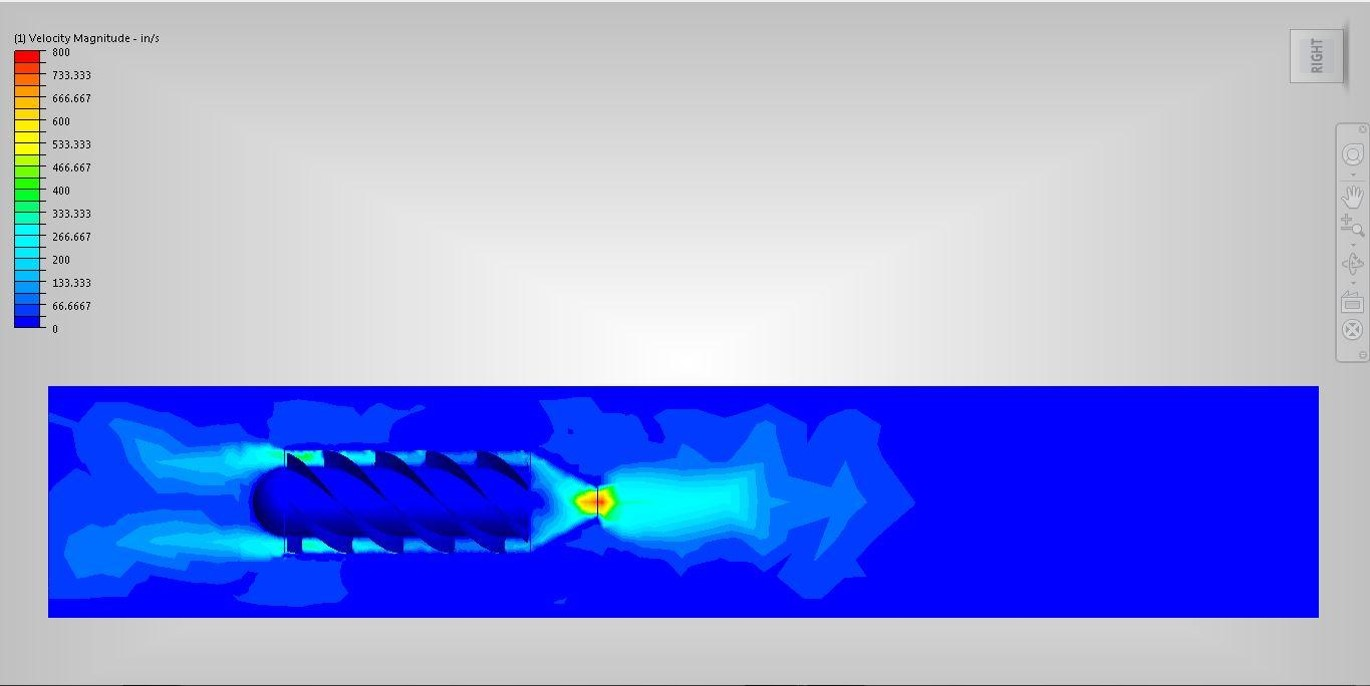
\includegraphics[width=12cm]{CFDvsbn}
\caption{CFD Analysis of the Vane Shell and Body  with the Nozzle} 
\end{figure}
The CFD analysis shows a maximum velocity right at the nozzle where it would be expected, however there is still a large area of recirculation and low velocity at the end of the vane shell. This reduces the total fluid velocity.
\paragraph{CFD Analysis of the Whole Propulsor Design}
The addition of the cone completes the propulsor design and removes the area of recirculation behind the vane shell. By removing this section the nozzle steadily converges the flow and increases its speed, sending a jet of high speed fluid out the back of the device. 
\begin{figure}[H]
\centering
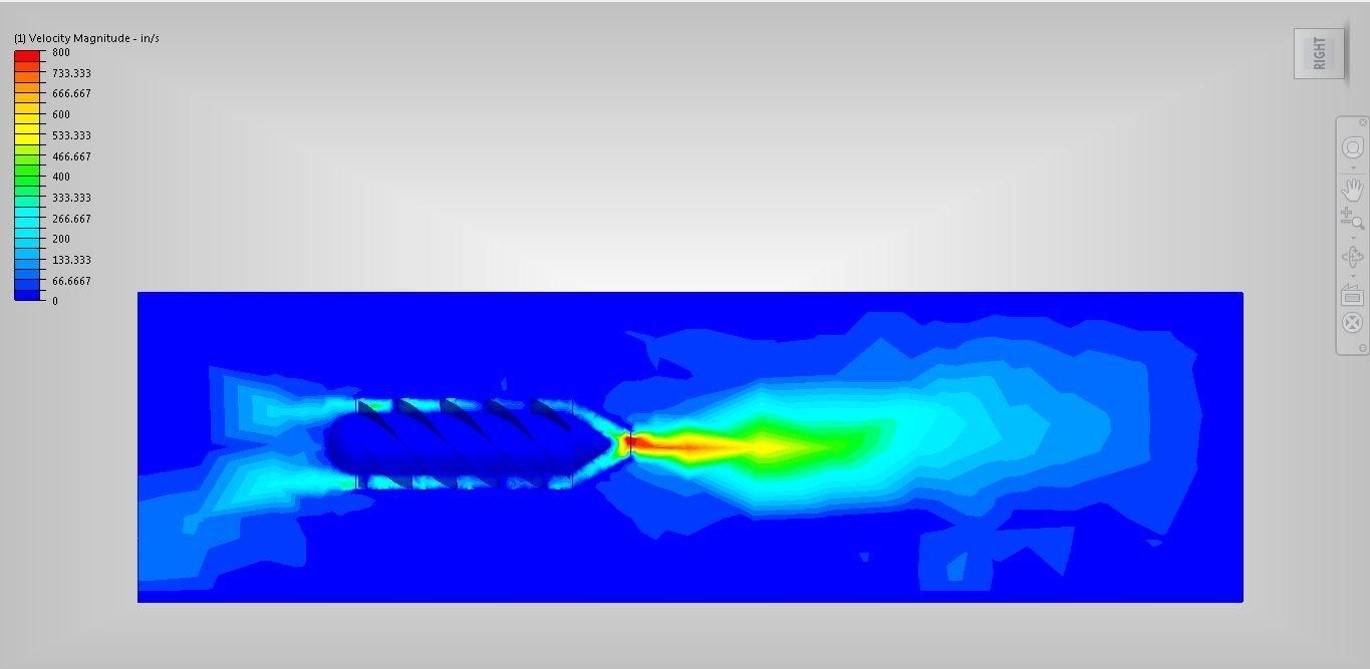
\includegraphics[width=12cm]{CFDvsbnc}
\caption{CFD Analysis of the Entire Propulsor Design} 
\end{figure}
	As seen in the figure the high speed jet of fluid generates the thrust that propels the vehicle through the water.
\subsubsection{Manufacturing}
The complicated geometry of the vane shell presented a challenge for manufacturing due to our limited resources. Any form of traditional manufacturing via removal of material, such as CNC milling or lathing, presented to high of a cost. Aluminum would be used for these methods due to the development of a protective Aluminum Oxide coat in a corrosive environment as well as the materials ease of manufacturing. \par
Selective Laser Sintering, SLS, was also considered due to the ease of production for complicated geometries. This method would be expensive, but has a shorter lead time than traditional manufacturing. This process would also produce a metal part. Metal parts would be significantly heavy, which would remove some of the need for permanent balast, however it would add a significant inertial load to the drive train.\par
Using an ABS 3D printer was also considered. This process had the lowest cost and lead time. There were some concerns about the strength of the part and the fact that it was quite large. Some further analysis was done on the part and was found that the loads would be low enough to be handled by the ABS. The vane shell was broken into six identical pieces so that it would fit within the print volume. \par
\begin{figure}[H]
\centering
\includegraphics[width=10cm]{"Vane Shell Von Mises Isometric"}
\caption{Isometric View of the Von Mises Stresses on the Vane Shell} 
\end{figure}

The Cal Poly Chapter of the Southern California Engineering Technologists Association, SCETA, was chosen to manufacture these six sections that comprised the vane shell.  Once these parts were received they were linked together using aluminum rods along the length and marine epoxy on the surfaces. This provided a strong bond between each of the six pieces. Once the epoxy had hardened the surfaces were sanded to remove epoxy overspill and printing errors. Then the entire surface was coated with ABS cement to smooth the surface, ensure bonding, and fortify strength.
\subsection{Body}
\subsubsection{Initial Considerations}
One of the major subsystems highlighted for improvement in Phase III of the project was the body.  In Phase I the body was really not a subsystem at all, but rather a section of 8” HVAC ducting that only serves to position the vane shell and constrain the flow through it.  For a vehicle that was to be stealthy, maneuverable, and capable of higher speeds, this clearly would not suffice and so a new streamlined body was to be a major focus of Phase III.\par
From the beginning of the project (even in the ideation and concept development that took place about four years prior to the start of Phase I), the vehicle was always a major focus and was meant to be advanced  both scientifically and aesthetically; however, simple streamlining was far from the only goal for the body.  In fact, the body really has a whole list of vital parameters pertaining to its design, a short sampling of which is included below:
\begin{itemize}
\item Streamlining for better performance
\item Ease of manufacture
\item Choice of materials
\subitem Ease of manufacture (repeated)
\subitem Cost of manufacture
\subitem Effect on the flow
\subitem Structural support (supports all other subsystems of the vehicle)
\subitem Weight (ease of transportation as well as buoyancy considerations)
\item Incorporation of flow control measures
\item Incorporation of stability measures
\item Stowage area/volume constraints
\item Permanent ballast (for decreasing buoyancy)
\item Free flood space (for decreasing buoyancy)
\item Thermal/magnetic/acoustic shielding
\end{itemize}
and the list goes on.
With regards to the actual shape of the vehicle as it related to streamlining, the original shape was purely influenced by a sense of biomimicry in that it was always meant to look like some sort of fish; this was for two main reasons:
\begin{enumerate}
\item Fish have been already optimized through natural selection and so rather than starting from nothing, it would cut down on work and improve the caliber of the final design significantly if the vehicle were to be designed within the framework of a biomimetic solution.
\item As has been documented previously in this report, one of the mission objectives is to produce a design that exudes stealth, at least in part with regards to inconspicuousness.
This design intent can be seen below both in the conceptual hand drawing that was produced near the end of Phase I and in the SolidWorks “Future Vehicle Concept” model below that was developed at the same time.
\end{enumerate}
\begin{figure}[H]
\centering
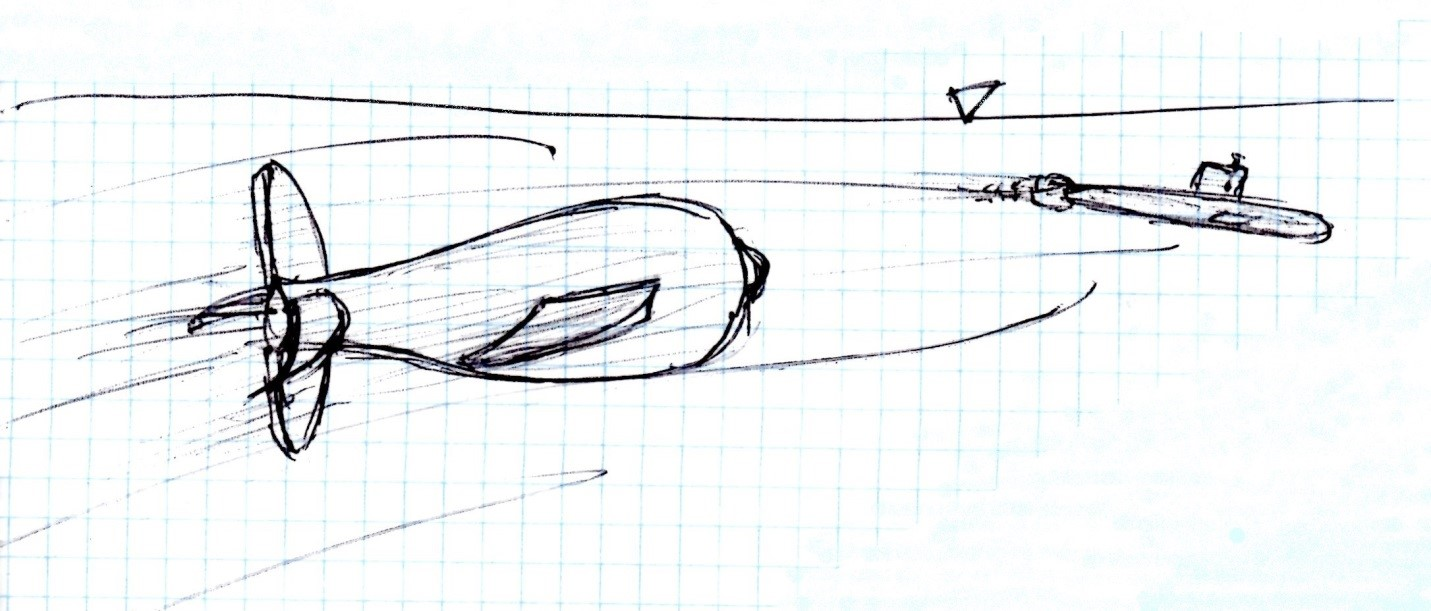
\includegraphics[width=12cm]{concept}
\caption{Conceptual Hand Drawing}
\end{figure}
\begin{figure}[H]
\centering
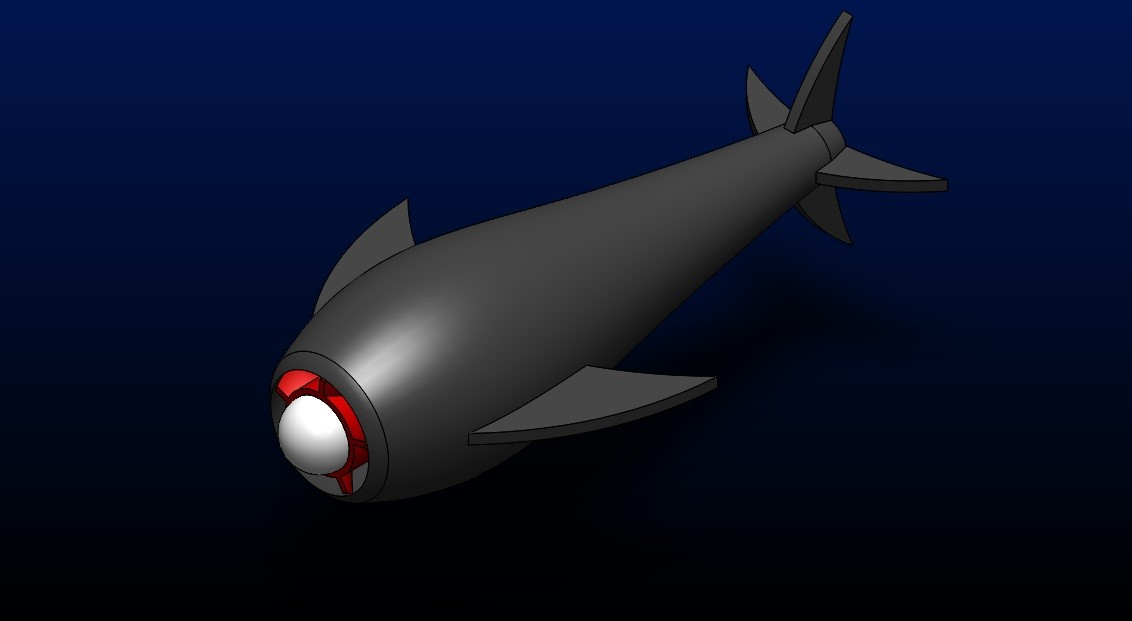
\includegraphics[width=12cm]{future}
\caption{A Possible Future Vehicle Design}
\end{figure}
The next step that followed in the design process after this ideation phase was the general practicality parameters.  This essentially began with an overall estimated desired size for the vehicle, which was set to be roughly the size of a scuba tank as this was seen as a size that would allow for all of the components to be fit into the body while still keeping the vehicle relatively portable.\par
Following this the next step was to start nailing down the manufacturing process, as the part would obviously need to be custom made and this introduced a large deal of complexity to the project, while also augmenting projected costs and imposing more stringent cost constraints.  As a first approximation to the build solution, additive manufacturing and CNC quotes were sought purely to get an idea of what it would cost to have it made professionally (rather than by the team), as having it made professionally would significantly decrease manufacturing time and help to produce a much more polished solution; additionally, this would serve as a jumping off point with regards to both developing an idea of how much it would take for the team to make it ourselves and to how high we should set our fundraising goal, as will be discussed later.  After receiving quotes for everything from aluminum CNC to injection molding to polyurethane casting, it was found that a professional build would cost anywhere from \$4k to \$10k; obviously this was completely unrealistic, but it served to shine some light on what kind of manufacturing processes the team should look at as well as the materials associated with the processes. \par
\subsubsection{General Body Shape}
Following this, a few different body styles were created in SolidWorks as conceptual studies to inter-relate location and size of propulsor, control surfaces, pressure hull, sensor suite, and buoyancy control.  A few sample designs can be seen below.
\begin{figure}[H]
\centering
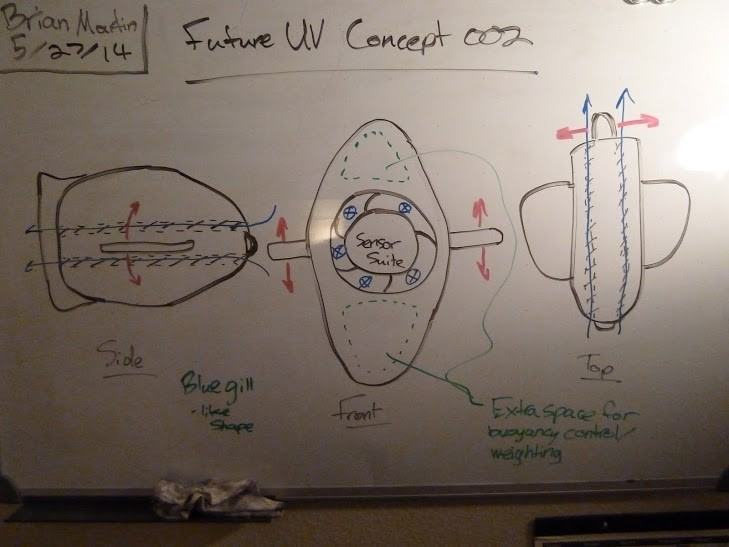
\includegraphics[width=8cm]{future2}
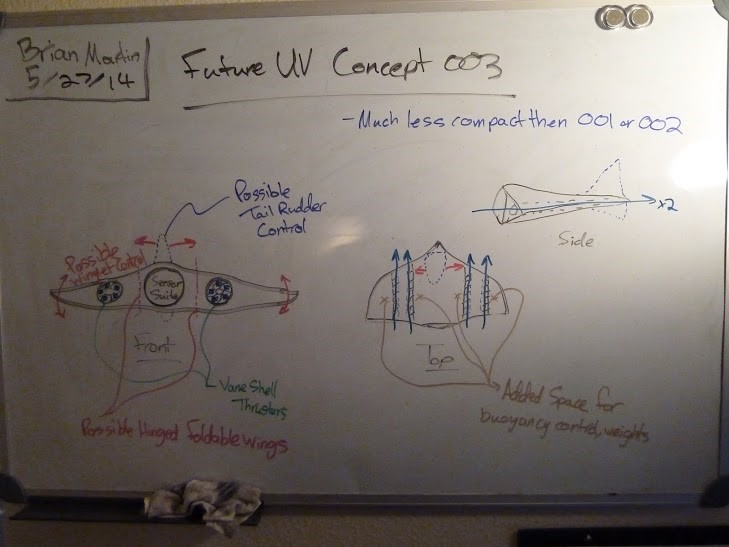
\includegraphics[width=8cm]{future3}
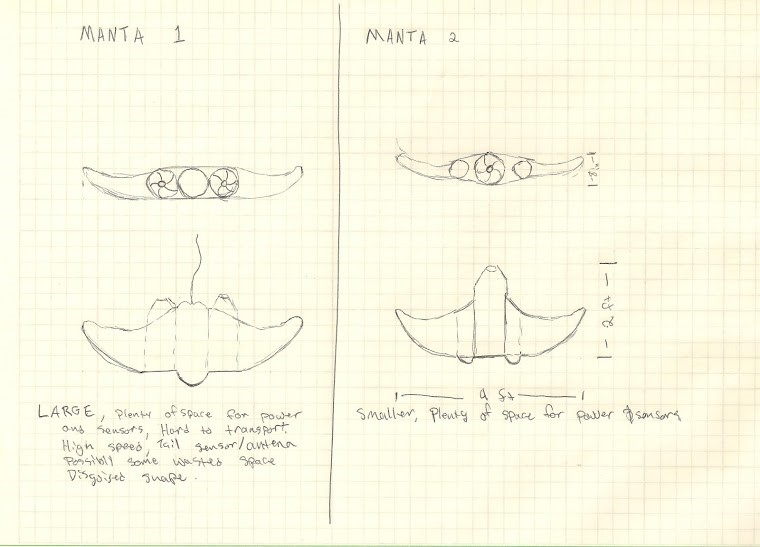
\includegraphics[width=8cm]{manta}
\caption{Possible Body Shapes for Future Design}
\end{figure}
Eventually it was decided that it was best to stick to the original design due to the stability, associated external hydrodynamics, internal stowage capabilities, and overall maneuverability (rising and falling movement is strongly influenced by the buoyancy control and thus is less of a concern, but movement in the horizontal plane is dependent more on the control surfaces, therefore if the vehicle is excessively tall, wide, or has a less than optimal slenderness ratio, rolling and yawing can become inhibited).
\subsubsection{Solid Modeling and Computational Fluid Dynamics (CFD)}
At this point the SolidWorks model of the entire assembly was coming together and so as the assembly became more complete, the body had to be adjusted repeatedly in order to get all of internal components to fit within the body while also keeping the vehicle relatively slender and tight against the internal components as excess volume would mean more positive buoyancy that would need to be combated using more permanent ballast and/or free flood space as well as a negative influence on vehicle maneuverability.  This process of sizing was repeated multiple times over the months leading up to (and into) the start of manufacture.\par
With the body shape and size essentially set, CFD studies were performed to validate the hydrodynamic integrity of the design.  Initially this led to more redesign due to issues such as recirculation regions, possible flow separation/reattachment, and other turbulent phenomenon.  Eventually the body got to the point of showing promising streamlining as shown in the below CFD image.
\begin{figure}[H]
\centering
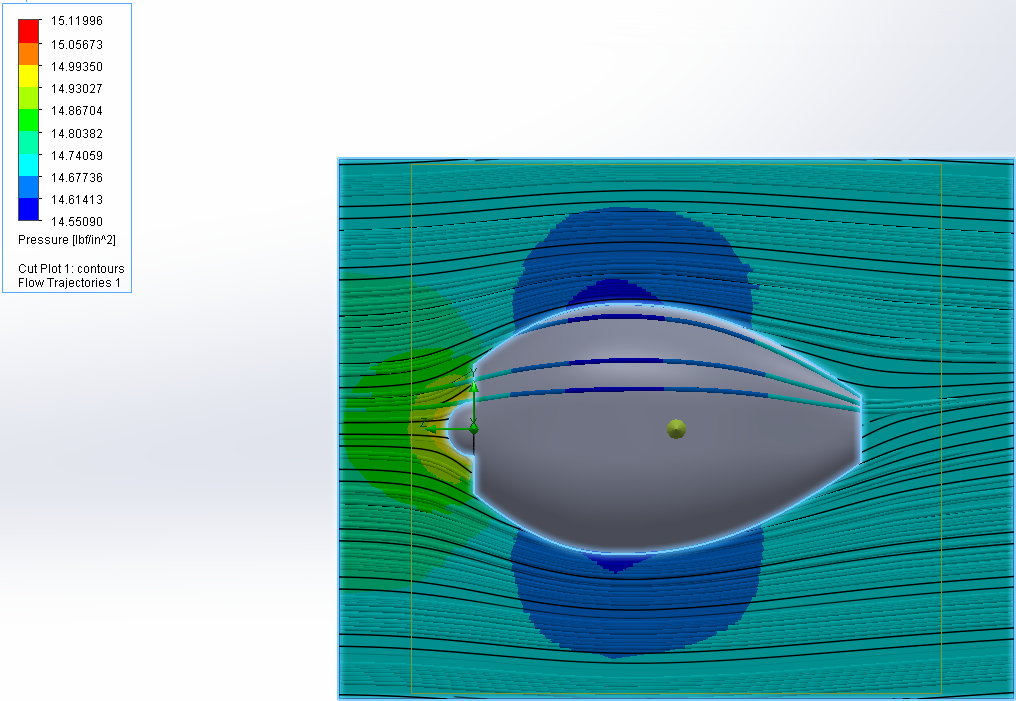
\includegraphics[width=12cm]{cfdbody}
\caption{CFD Analysis of the Body}
\end{figure}
An interesting note to make is that the position of the dome forward from the body actually has a significant effect on the flow in that a stagnation point exists at the tip of the dome providing higher pressure for enhanced fluid acceleration into the inlet, helping to overcome initial chop created by the vane leading edges.
\subsubsection{Materials \& Manufacturing}
With the final design completed and the manufacturing period fast approaching, a body mold had to be created and materials had to be selected.\par
For the body mold, the body solid model had to be re-created in SolidWorks using a multi-level loft.  Next the actual cross sections of the loft were printed out to full scale and then used to make cardboard cross section cutouts which were then inserted into a large foam block at regular precisely sized intervals corresponding to the lofting in the solid model.  Next a maximum height profile was also printed out and used to cut a cardboard piece that was mounted to the side of the foam. Next this max height profile was used to remove large chunks of material from the foam block, yielding the proper axial curvature. \par
\begin{figure}[H]
\centering
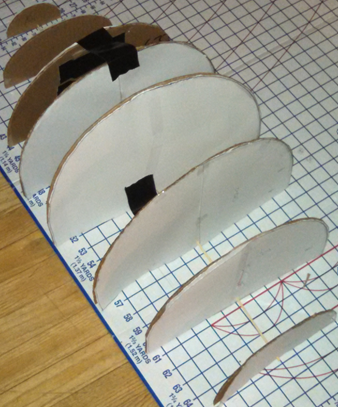
\includegraphics[width=6cm]{contours}
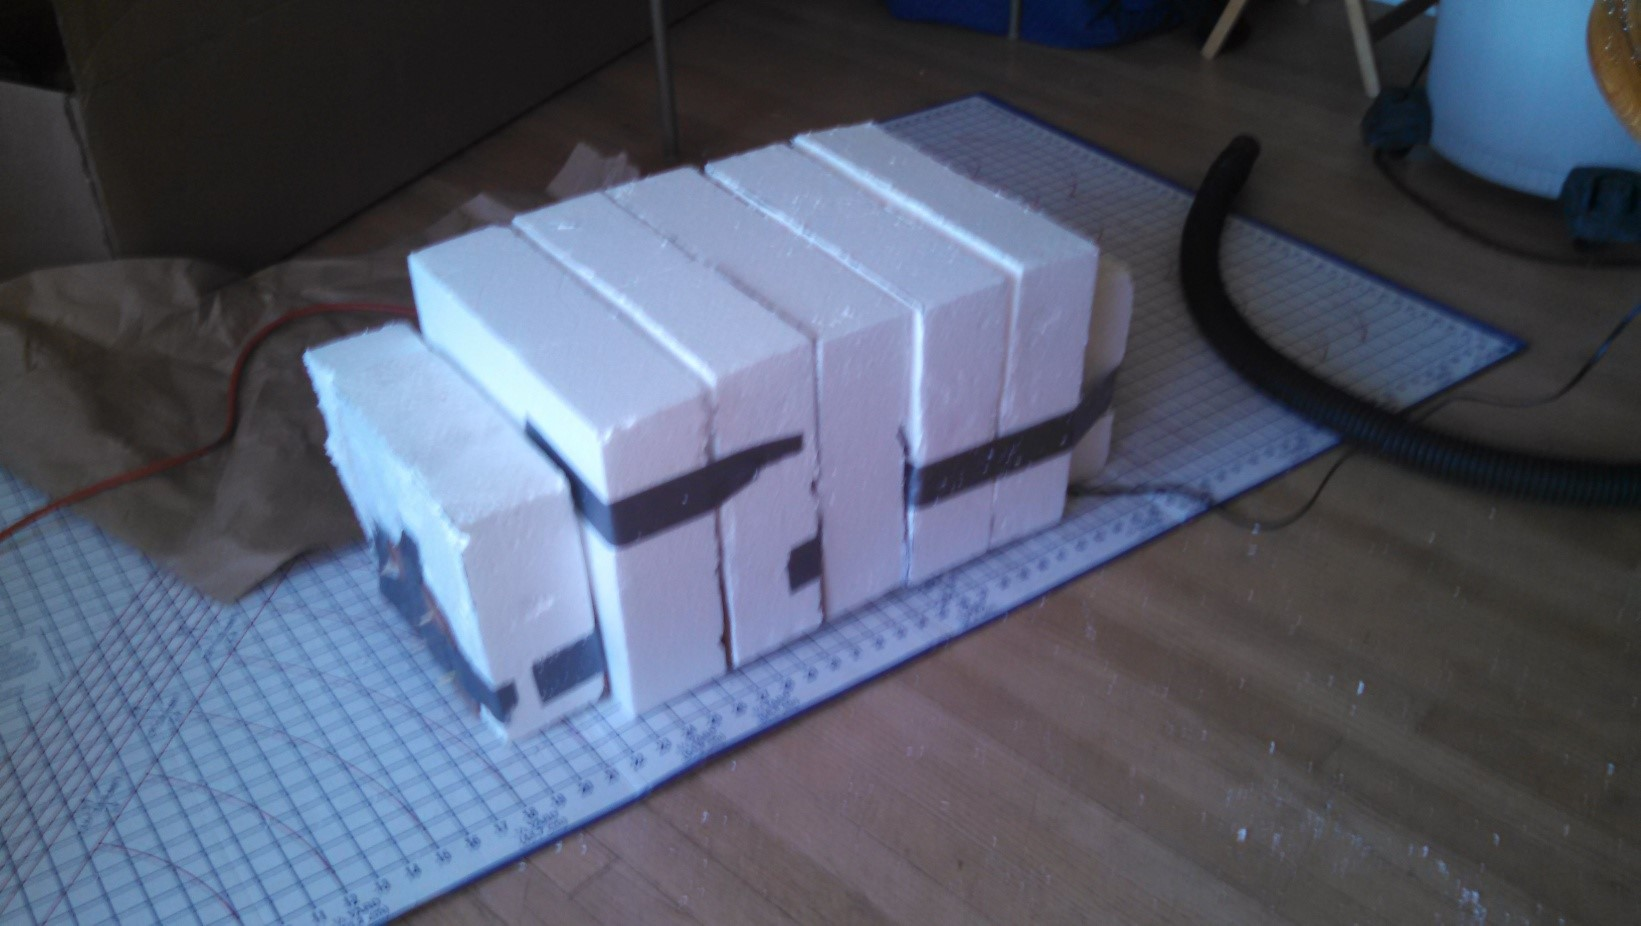
\includegraphics[width=8cm]{foam}
\includegraphics[width=8cm]{cutfoam}
\caption{Creating the Foam Mold for the Body}
\end{figure}
Now the max heights profile cardboard was removed and the cross sectional rounds were used to further whittle down the body foam  using a combination of a hot wire cutter, bone saw, and bread knife.  This process was extremely time consuming and consisted of one member slowly shaping the body and checking streamlining by eye for about six hours straight until the original visualization of the body was recreated.
\begin{figure}[H]
\centering
\includegraphics[width=12cm]{wrappedfoam}
\caption{Final Mold Ready for Body Creation}
\end{figure}
At this point the body mold was wrapped in wax paper pieced together with duct tape in order to keep any molding material from sticking to the foam.  Now that the body mold was built, it was time to move on to the material for the body itself.\par
Originally carbon fiber had been looked at due to structural, moisture, and aesthetic properties, but due to price point, the team moved on to considering other materials.  Eventually the team looked into casting materials and found a Smooth-On Smooth Cast 385 mineral filled polyurethane casting material.  This specific casting material was selected based on its strength, moisture properties, curing time, impact resistance, ability to be colored, and viscosity (if it was not viscous enough, it could drip during the casting process).  In order to deal further with possible viscosity complications, it was decided that the body mold would be made out of cardboard and Styrofoam and that we might design in ridge-like bulkheads to confine dripping material to quadrants.
\begin{figure}[H]
\centering
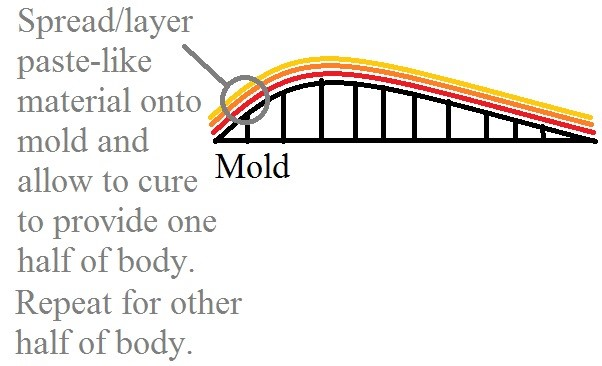
\includegraphics[width=10cm]{fglass}
\caption{The Body Manufacturing Process}
\end{figure}
Upon receiving and testing the material, it became clear that the material was much more brittle than we thought and that it would require at least 0.5 in wall thickness to toughen up the material, but even then there was major concern for when we drilled into the body (poor machinability due to the brittleness) to mount servos for the control surfaces as well as for how we would fix the two halves together (original idea was to drill in some sort of hinge).\par
To remedy this we tried to reinforce the material with cut up strips of old t-shirts, which actually worked pretty well; however, there was still concern about maintaining even thickness and because it took a long time for it to cure, there was a chance we could invest a lot of time and still end up with something that didn’t work.  So we decided to move on to using heat moldable ABS sheets.\par
First off, we ran to the local hardware store and both pipe end caps made out of ABS both 1/8 in and 1/4 in thick and conducted informal impact testing with a sledge hammer to see the difference between the ABS and the casting material; the casting material shattered with hardly any impact, but the ABS took whatever impact was thrown at it…even literally when we conducted “throw-against-the-wall-really-hard impact testing” of both materials.  Additionally, we tried to heat form them using 1500W heat guns and quenching them in place with water.  This system worked relatively well and so we went ahead and bought 2 large panels of ABS that could be used form each side of the body; unfortunately, when the material showed up it was actually $1\over4$ in thick, but we did not have time to re-order the material and thus went ahead trying to form it to our mold.  First we tried with two handheld 1500W heat guns but found that we were losing heat to the environment at too rapid of a rate, so we built a tin-foil lined cardboard and plywood enclosure with two holes for the heat guns at the top.\par
\begin{figure}[H]
\centering
\includegraphics[width=10cm]{hotbox}
\caption{First Attempt at an ABS Forming Box}
\end{figure}
This worked well for about 10 minutes and was partially deforming the ABS, but the heat gun nozzles began to melt (they were poor quality bought from Harbor Freight for about \$15).  The ABS had already partially formed though, so we removed the heat guns and ducted the heating element of a propane patio heater into the makeshift oven.
\begin{figure}[H]
\centering
\includegraphics[width=10cm]{hotbox2}
\caption{Second Attempt at an ABS Forming Box}
\end{figure}
This only worked for about 5 minutes as the heat was greater and the duct tape all melted; as a last ditch effort we tried using butane blow torch for localized deforming, but due to the thickness and large size as compared to the small flame, the ABS began to vaporize and the ABS sheet could not deform on a large scale.\par
At this point, a family member of the team informed us that he could get fiberglass for relatively cheap and so we decided to go back to the original idea of using composites.  Prior to using the fiberglass, the body mold was wrapped in a few layers of duct tape since the fiberglass resin reaction is exothermic and we did not want to risk the body mold melting.  Over the next few weeks we worked on building up the fiberglass and adding resin then sanding back in order to get the body nice and smooth with plenty of structural integrity at about a 0.5 in sidewall.
\begin{figure}[H]
\centering
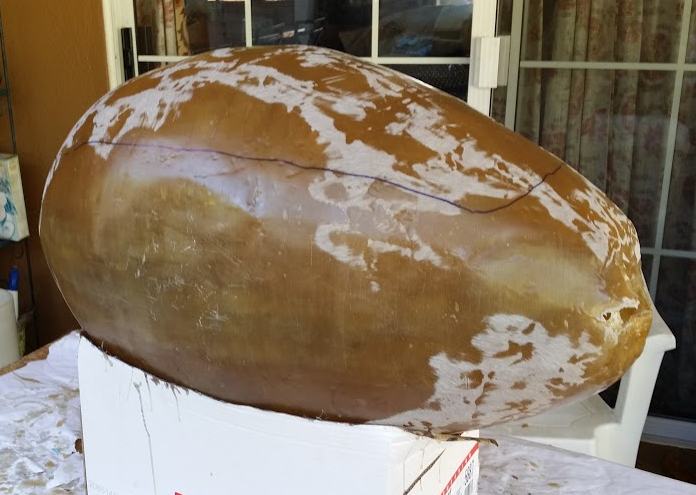
\includegraphics[width=10cm]{finishedFglass}
\caption{The Fiberglass Body}
\end{figure}
The next step was to integrate the propulsor subassembly into the body at which point we first cut a lid out of the top of the body and took a long time to center the drawn holes and then drilled the 8” entrance hole and 2.25” exit hole and seated the body cylinder into the front hole and the axial gap between the nozzle and the aft body hole was bridged with a straight aft extension coupler.  Before everything was locked into place, the body mold was reused by cutting it down significantly and using it to support the weight of the body cylinder/propulsor subassembly.  This worked perfect for this purpose since it already conformed to the shape of the body.  Once the foam was cut to the right height, a cavity was cut out of the foam to house the batteries and a cardboard door was added to protect the waterproofing of the batteries from getting snagged on metal.  Lastly all of the foam and cardboard was wrapped with duct tape to keep it from getting damaged in the case of a leak.
\begin{figure}[H]
\centering
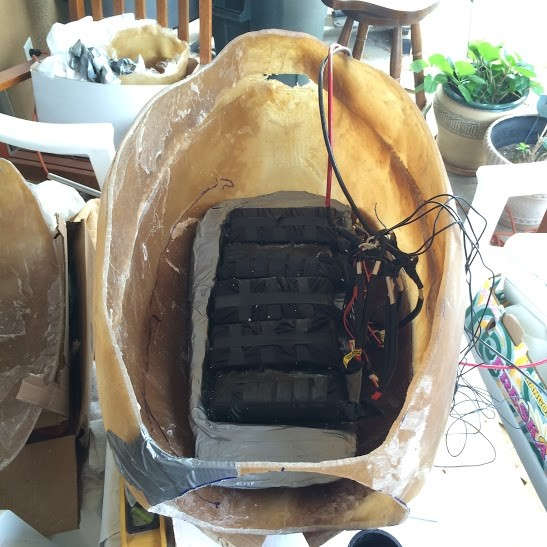
\includegraphics[width=10cm]{openFglass}
\caption{Batteries Seated in the Fiberglass Body}
\end{figure}
This foam support was then locked into place with silicone form-a-gasket and then used fiberglass, marine epoxy, and silicone caulking to seal the body cylinder, nozzle, and straight aft extension coupler into place on the body.\par
The next step was then to carefully over a long period of time align all of the servo mounts, servos, and control surface hardware into their appropriate places of the body and then drill tight fitting holes in the body to mount up the control surfaces using fasteners and marine epoxy.  Lastly, a hole was drilled at the base of the body to route the buoyancy control to a lower section of the body using polyurethane hosing since while surfaced, the body would not be able to pull in water from above the waterline; this hole was also epoxied around.
\begin{figure}[H]
\centering
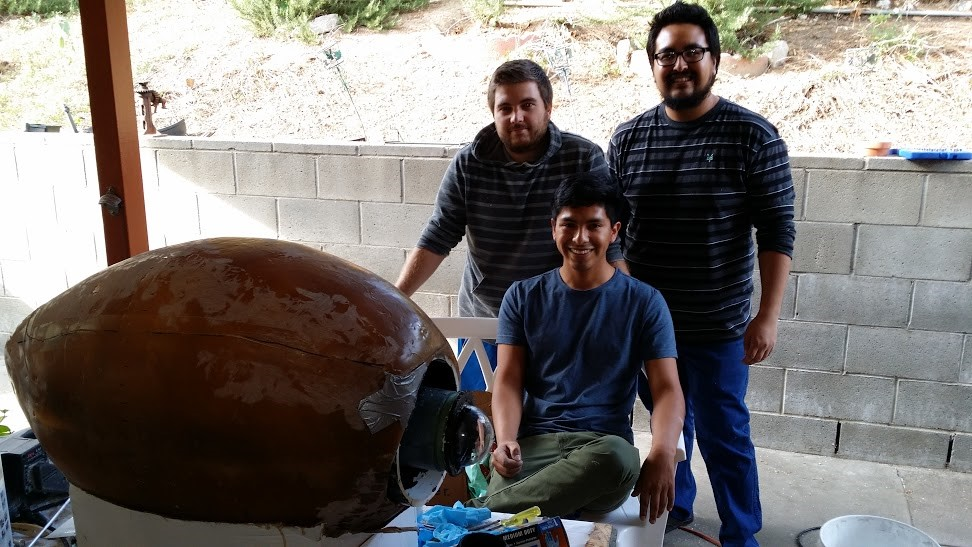
\includegraphics[width=10cm]{teamFglass}
\caption{The Final Body}
\end{figure}
Once ready for testing, the permanent ballast will be configured by setting the vehicle in the water and continually adding weight until neutral buoyancy is reached and the buoyancy control system is capable of bringing the vehicle up and down in the water column.\par
The last step was to spray paint the body black to lower its observable visual signature and then, after some testing, to apply the superhydrophobic coating to observe its effect on drag reduction.
\subsection{Control Surfaces}
\subsubsection{Hydrofoil/Airfoil Design}
The purpose of including control surfaces into the vehicle design was to add maneuverability. They would ultimately control roll, pitch, and yaw for the vehicle by a combination of biomimetic pectoral fins and tail fin. Initially, the team designed an original foil shape, as seen in Figure 1. This design was arbitrary as it only served as an example to run CFD analysis, however, the pressure distribution at the leading edge would cause excessive drag as it was too bulbous.  It was decided to use a hydrofoil/airfoil found in a UIUC Airfoil Coordinate Database as CFD results for lift force and torque the vehicle would experience were more reliable also seen in the figure. 
\begin{figure}[H]
\centering
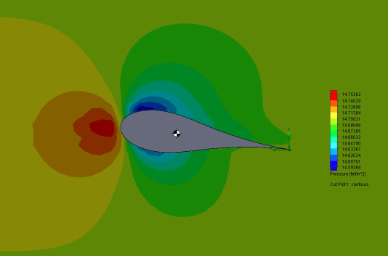
\includegraphics[width=8cm]{hfl}
\includegraphics[width=8cm]{hfr}
\caption{(LEFT) Original team designed airfoil, (RIGHT) UIUC airfoil.}
\end{figure}
The control surfaces were designed using a symmetric foil as opposed to a cambered geometry that most airplanes use. The reason for this was to not create lift fluid forces when the angle of attack is at 0$^\circ$ relative to the axis of propulsion of the UV.  Also, the control surfaces would be operating at lower angles of attack (up to about $\pm12^\circ$) both symmetric and cambered airfoils would produce near identical amounts of lift.  With this design criteria in mind the vehicle would be able cruise at a certain plane of depth without moving vertically. The EPPLER E838 HYDROFOIL AIRFOIL (e838-il), seen in the below Figure,  was chosen for the design of the two pectoral fins and the tail fin and their angle of attack would be controlled by revolute servos. Servos were chosen over stepper motors because of the accurate feedback on position that servos provide.
\begin{figure}[H]
\centering
\includegraphics[width=12cm]{eppler}
\caption{EPPLER E838 HYDROFOIL AIRFOIL (e838-il)}
Courtesy of: http://airfoiltools.com
\end{figure}
\subsubsection{Design of Control Surfaces}
Originally, the control surfaces were designed to have moveable flaps via a rotary shaft driver assembly, as seen in the following two figures, which would only control the trailing edge much like the design of ailerons on airplanes.
\begin{figure}[H]
\centering
\includegraphics[width=8cm]{cso}
\caption{Original Control Surfaces Idea with Flaps}
\end{figure}
\begin{figure}[H]
\centering
\includegraphics[width=8cm]{Hinge}
\caption{Rotary Shaft Driver Idea Design}
courtesy of: http://www.irfmachineworks.com
\end{figure}
However this design was abandoned as it would put high torque loads on the flaps themselves which would increase the cost of the servos as they would have be larger and  rated for a much higher holding torque. It was later decided that the entire control surface would revolve around of the axis of rotation of the servo and through the, as seen in the following figure, center of mass of the control surface and an angled driver shaft would transfer torque. 
\begin{figure}[H]
\centering
\includegraphics[width=8cm]{ttcs}
\caption{Torque Transfer for Control Surfaces}
\end{figure}
This would theoretically cancel out most reactant torque couples that the control surface would experience from incoming flow of water, making the design holding torque for the servos much lower than originally planned. Generic High Torque Servos (rated at about 5.2 lb-in of maximum deliverable torque) were chosen control the surfaces. The shape of the control surfaces was biomimetic in terms of geometry as it tapered away from the body, was curved at both the leading and trailing edge, and ended at point almost resembling a shark’s pectoral fin as seen in the following figure. They would be 3D printed in ABS, for its corrosion resistance and high fracture toughness, in two parts and marine epoxied together and coated with ABS cement to strengthen and fill in voids and discontinuities that may have occurred in manufacturing.
\begin{figure}[H]
\centering
\includegraphics[width=8cm]{csbw}
\caption{3D Printed Pectoral Fin Control Surface}
\end{figure}
\begin{figure}[H]
\centering
\includegraphics[width=8cm]{cscfd}
\caption{CFD of pectoral fin with surface plot of flow trajectories.}
\end{figure}
The tail fin (rudder) was designed using the same foil as mentioned above but larger and angled near the base to avoid seizing with the body of the vehicle upon changing angles of attack. Unfortunately due time and size constraints in 3D printing, the design could not be manufactured the same way as the pectoral fins. Instead, the geometry was cut out from three sheets of $1\over4$” ABS and fastened together using threaded screws as seen in the following figure. Then it was coated with ABS Cement to increase smoothness and fill voids and discontinuities. 
\begin{figure}[H]
\centering
\includegraphics[width=8cm]{rudder}
\caption{Rudder shape cut out on paper positioned on sheet of ABS}
\end{figure}
\subsubsection{Control Surface Assembly}
For the pectoral control surfaces, servos were fastened onto 3D printed ABS mounts, as seen in Figure 9, which would mate with to the outer surface of the body cylinder. Marine epoxy would be used to fix the mounts at the theoretical center of mass of the vehicle, perpendicular to the vertical line of symmetry, on both sides of the vehicle.
\begin{figure}[H]
\centering
\includegraphics[width=12cm]{servomounts}
\caption{3D printed ABS servo mounts}
\end{figure}
The rudder however would have the servo epoxied directly to the straight aft extension coupler as time constraints did not allow for a 3D printed mount like the pectoral fins. The angled shaft was made of precision ground 0.25 inch 6061 aluminum rod mainly due to the oxide layer that would form when the rod was submerged, allowing it to passivate and not corrode any further. The shafts would mated to the servo’s spline via a shaft coupler made of 316 stainless steel. A 0.25 inch steel ball bearing was added to the assembly to react to any misalignment or deflections that shaft might experience in positioning and/or operation to avoid applying that load to the body entirely. A graphite-reinforced, spring loaded, corrosion resistant PTFE shaft seal was used to seal out water due to its high corrosion resistance and high maximum pressure resistance (250 psi) for slow rotary motion of the control surfaces. The maximum amount of operational hydrostatic pressure the seal would experience would roughly be around 30 psi but the dynamic load was still unknown during the design phase so a 250 psi rated shaft seal was the best choice for the price allowing for a high factor of safety to account for the unknown maximum pressure. The shaft seal and ball bearing were set into a 3D printed cylindrical mount that would be epoxied to a bore in the wall of the body of the vehicle. 
\begin{figure}[H]
\centering
\includegraphics[width=8cm]{servoshaft}
\caption{Control surface assembly: servo, shaft, ball bearing, and shaft seal.}
\end{figure}
\subsubsection{Further Development of the Control Surfaces}
The final size of the control surfaces were about 30\% smaller than originally desired. This was due the size of the control surface being incorrectly dimensioned for the size of the propulsor, not the overall length of the vehicle which includes the straight aft extension coupler and nozzle. 
\subsection{Buoyancy Control}
The underwater vehicle was designed to be neutrally buoyant. Therefore the need of a device to control the device to dive deeper into the water or rise to the surface was important. Buoyancy force is determined by the following equation Fb = ρ x g x V. Since the density of the water does not change significantly with respect to depth the team decided to change the density of the device itself by changing it mass by using a piston ballast tank. The piston ballast tank is made by the company Alexander Kengel KD located in Germany. Components of the ballast assembly are the following: 12V motor, threaded rod with piston, gear reduction system of 15:1, hollow metal cylinder, and limit switches. The main function of the ballast tank is to intake and expel water to control the buoyancy of the underwater vehicle. Voltage is ran through the motor that is connected to the gear reduction system. The gear reduction system is attached to the threaded rod and with rotational power given from the motor displacement of the threaded rod occurs to expel or intake water. A figure of the device is seen below.
\begin{figure}[h]
\centering
\includegraphics[width=8cm]{bcOverview}
\caption{Overview of the Buoyancy Control Device}
\end{figure}
The ballast tank itself can intake up to 30.5 cubic inches with an overall length of thirteen inches.  When the correct voltage is applied the tank can go from full stroke to no stroke in eleven seconds.  Limit switches (white components seen in the figure above) are used to determine the position of the threaded rod and piston assembly. One limit switch will indicate that the piston is located at the halfway point. The other limit switch is to indicate the piston has been fully retracted and shuts off power to the motor to ensure no damage to the ballast tank occurs. The piston ballast tank is suitable up to a depth of 34 feet. This piston ballast tank assembly is connected to the brains of the device to submerge the underwater vehicle where depth can be measured by the accelerometer.  Once depth is achieved the vehicle will be able to run its mission. The dimensions of the ballast tank can be seen in the figure below. Dimensions noted in figure are in millimeters.
\begin{figure}[h]
\centering
\includegraphics[width=8cm]{bcDetails}
\caption{Details of the Buoyancy Control Device}
\end{figure}
\subsection{Pressure Hull}
Drawing from the concept found in SHEILA-D, the pressure hull is used to house vital components that power the project.  Located at the center of the vehicle, within the vane shell, the pressure hull was designed to satisfy numerous challenges associated with underwater operation.  After seeing how vulnerable SHEILA-D was to flooding, we knew that limiting entry points and creating obstacles for any water that may leak in was of top priority.  Our new design of powering the vane shell through a shaft located at the rear of the pressure hull eliminated the need to cut holes into the PVC pipe to transmit power.  This left the two pipe openings at either end and any holes needed to pass communication and power wires to external actuators.
\begin{figure}[H]
\centering
\includegraphics[width=8cm]{"Pressure Hull"}
\caption{The Pressure Hull Design}
\end{figure}
The front of the pressure hull was slightly redesigned to allow for better sealing and the integration of a smaller, micro-controlled camera.  A dome was ordered off the shell and mated to a PVC end cap using marine epoxy and then covered in ABS cement for good sealing measure.  To allow for easy access to the camera, a custom hinged door was then fabricated onto the back of the domed front cap.  Upon ending a session and removing the cap, the SD card containing video footage could be easily ejected without hassle.  The front cap can then be slipped on and sealed with silicone for non-permanent but water proof sealing.
\begin{figure}[H]
\centering
\includegraphics[width=8cm]{"PHFront"}
\includegraphics[width=8cm]{"CameraDome"}
\caption{(LEFT) Dome Front Cap fixed to the pressure hull. (RIGHT) Inside Cap Camera Door}
\end{figure}
Five holes were cut at the front of the pressure hull, along the circumference, to do two things: run wire to external electronics found within the body and rigidly connect the body to the pressure hull.  The holes were mated to a matching set found on the body cylinder and the two sets were then connected by aluminum standoffs.  Wires from the logic command center could then be routed to the control surface servos, buoyancy control subsystem, and battery bank safely avoiding contact with water and the rotating vane shell.  The main purpose for the standoffs was to address the torque transfer issues from Phase 1.  We noticed that when rotating the vane shell in SHEILA-D, the torque transmitted to the vane shell would also cause the pressure hull to rotate relative to the body cylinder.  Rigidly connecting the body and pressure hull cylinders would keep them oriented properly and allow for full energy transfer to the vane shell.  Locking the body and pressure cylinders relative motion also keeps our wiring safe from being pulled in any one direction which could disconnect important navigational actuators or tear the wires completely.
\begin{figure}[H]
\centering
\includegraphics[width=8cm]{"standoffs"}
\caption{Wire standoffs before being trimmed of excess material.}
\end{figure}
The middle of the pressure hull is the home of Dory’s logic command center which includes an Arduino Uno, IMU, SD card breakout board, and Sabertooth motor controller.  The electronics sit atop a hand-fabricated, aluminum slider tray aimed at high accessibility.  The tray is a two-piece assembly made out of C channels and flat plate aluminum stock with the track permanently fixed to the bottom of the pressure hull with marine epoxy.  Aluminum was chosen here to wick heat away from the electronics under heavy usage.  The tray is easily slid on and off the track to gain access to the logic command center between running sessions and when data is to be collected.  The tray is able to be removed 2 feet from the body fully wired and can be completely removed in a few steps.  The detachable tray is locked in place by rubber stoppers in the back and pressed in from the front by the front dome cap.  A fixed position was crucial in ensuring that the logic command center doesn’t slide around freely during underwater sessions as any unwanted movement in the tray can lead to disturbances in the IMU readings or even damage to electronics themselves.  The slider tray was then completed by the addition of a rubberized, aluminum handle which was fixed rivets.  The handle was incorporated to easily pull the tray out for data collection and protect the users in the case of electrical shock.
\begin{figure}[H]
\centering
\includegraphics[width=8cm]{"tray"}
\includegraphics[width=8cm]{"brains"}
\caption{(LEFT) Top view of slider tray. (RIGHT) Logic Command Center on slider tray. Note riveted handle.}
\end{figure} 
The rear of the pressure hull houses the driving motor for the vane shell and the motor mounts.  The motor mounts were designed to completely fill the inner circular area of the pipe.  Two mounts were 3D printed to support the motor and gearbox at two points with an annular open region between the two.  The motor mounts also would act as bulkhead as seen in many water or air based vehicles.  Bulkheads are walls that separate regions of a hull to minimize overall damage in the event of an accident.  In our application the bulkheads are used to block water from reaching the electronics package from the rear of the vehicle.  Water will have to reach the rear of the pressure hull by first going through the vane shell, vane shell coupler, and motor shaft seal, before reaching the bulkheads.  In the event that water gets through the first bulkhead, the second bulkhead will help contain the water.  The motor mounts are fixed to the vane shell by marine epoxy and sealed with silicone. \par 
To complete the package, the outer surface of the pressure hull is lined with three sets of plastic strips epoxied in place.  These strips are used to both space out the vane shell and provide a low friction surface for the vane shell to ride on.  Another strip of plastic is placed on the pressure hull which mates to the front of the vane shell to act as a thrust bearing, relieving some of the thrust load on the motor.  
\subsection{Drive Train}
The drive train in the assembly converts the electrical supply from the batteries into rotation motion for the vane shell. The Banebots RS-550 Motor provides 70.55oz-in (4.41 lbf-in) of torque and when coupled with the Banebots P60 Gearbox gearbox provides 4515.2oz-in (282.2 lbf-in) of torque to be transferred to the vane shell. The reason for designing the vehicle with such high torque was to ensure that any resistance to rotation, whether due to traction or due to inefficiencies from manufacturing, would be overcome.
\begin{figure}[H]
\centering
\includegraphics[width=8cm]{gearbox}
\caption{Banebots P60 Gearbox. Courtesy of: robotshop.com}
\end{figure}
3D printed ABS mounts were used to concentrically fix the motor and gearbox to the pressure hull. The mounts served as bulk heads to seal water out of the pressure hull section that contained vital electronics. A Stretch-Fit Rotary-Shaft Seal was also used in conjunction with marine grease to seal water from getting into the gearbox as seen in the following figure. A 3D printed ABS flange coupler was mated and epoxied to the gearbox shaft and to the vane shell’s inner diameter to transfer torque to the vane shell. The design of the torque transfer assembly used epoxy intentionally to create a semi-rigid connection rather than a rigid connection.  If the vane shell were to seize during operation, the epoxy bond would be the first to fail rather than the motor or vane shell which are both costly to repair and replace.  
\begin{figure}[H]
\centering
\includegraphics[width=8cm]{motormount}
\caption{Gearbox mounted to pressure hull and shaft seal attached to gearbox shaft.}
\end{figure}
The end of the shaft would rest and freely rotate inside the cone which would be rigidly fixed to the body cylinder. This would allow for support of the aft side of the pressure hull and to prevent erosion of the cone with a Lubrication-free Acetal Ball Bearing as seen in the following figure.
\begin{figure}[H]
\centering
\includegraphics[width=8cm]{cone}
\caption{Gearbox mounted to pressure hull and shaft seal attached to gearbox shaft.}
\end{figure}
\subsubsection{Future Drive Train Development}
A lower torque motor and gearbox are desired pending on testing and performance data of operational conditions of the vehicle.  The future design of the vehicle will move towards higher operational speeds to become more competitive with other UVs currently being developed.  Also, possible replacement of the Acetal Ball Bearing with a steel ball bearing would be wanted in future designs as the acetal would eventually erode and no longer be useful to support pressure hull.  
\subsection{Sealing}
\begin{figure}[H]
\centering
\includegraphics[width=8cm]{"loctite"}
\includegraphics[width=8cm]{"silicon"}
\caption{(Left) Loctite Marine Epoxy (Right) Silicone Sealant}
\end{figure}
One of the most challenging aspects in designing a UV is sealing against the environment for prolonged periods of time.  For our design we opted to use Loctite Marine Epoxy at all mating surfaces and potential water pathways.  Marine epoxy is formulated to bond wet surfaces and can be handled underwater in two hours.  After curing for 24 hours, marine epoxy dries to a final strength of about 3000psi[LOCTITE] with no shrinkage or expansion. Epoxy was applied throughout the entire vehicle but most heavily around the pressure hull to prevent water leaking into the sensitive electronics trey.  At mating locations where a permanent bond is not desired but water proofing is, silicone was the caulking of choice.  Supreme Silicone is water ready in 30 minutes and dries to a flexible, waterproof seal.  This was applied to the dome front cap before mating to the front of the pressure hull and around the body lid.  Lastly, ABS cement was used to fill in any gaps present on 3D printed parts.  Abs cement dries in 15 minutes and can be sanded to obtain any desired surface finish.
\subsection{Electronics}
A major leap forward from SHEILA-D is the integration of controls and electronics in Dory.  Our Phase I attempt was merely a 12V 2A LiPo battery undersupplying two powerful 12V DC motors with a switch to turn the motors on at full speed.  Not only was this not adequately safe for the user but it wasn’t safe for the vehicle.  During Phase II, our team set out to learn as much about electronics and controls of machinery as possible.  Our goal was to deliver a well-controlled vehicle with data collection capability that was much more sophisticated than SHEILA-D.    After becoming familiar with the world of Arduino and robotics, we applied our new found and self-taught knowledge to develop Dory’s Logic Command Center.  With a few choice parts, we were able to piece together an electronics package that can generate position and orientation data, save it to an SD card, record synced video, and control various actuators found throughout the vehicle.  
\subsubsection{Motor Controller}
\begin{figure}[H]
\centering
\includegraphics[width=8cm]{"sabertooth"}
\caption{Sabertooth 2x60 Motor Driver Courtesy of Dimension Engineering}
\end{figure}
Obtaining full control of the powerful vane shell motor is made difficult by the needs of the motor at stall.  The specific motor we chose consumes upwards of 80A at stall torque which is higher than any readily available motor controller on the market except for one.  The Sabertooth 2x60 Dual Motor Driver is the most powerful and user-friendly controller on the market today.  Each channel is capable of providing a burst current of 120A with normal operation around 60A; making it a perfect fit for our application since we will also be driving a DC motor to actuate the buoyancy controller.  Using the onboard DIP switches we used the driver in Simplified Serial mode to make coding as simple as telling the driver which motor channel to engage and at what speed to run the motor.  The Sabertooth also contains a 5V 1A Battery Eliminator Circuit (BEC) which drops the supply voltage low enough to drive the control surface servos.  Since servos have higher current draw than the logic board (Arduino) can provide, the Sabertooth fulfills two power needs in one package.
\subsubsection{Micro SD Card Breakout Board}
\begin{figure}[H]
\centering
\includegraphics[width=8cm]{"sd"}
\caption{MicroSD Card Breakout Courtesy of Adafruit.com}
\end{figure}
Adafruit supplied the Micro SD breakout board which worked perfectly for saving the data generated by the inertial measurement unit(IMU).  The board is driven directly by the Arduino’s 5V power supply and only uses four digital pins.  Once data is made ready by the IMU, a file is opened and saved to in a commonly found,  class four Micro SD card formatted to FAT32.  
\subsubsection{Camera}
\begin{figure}[H]
\centering
\includegraphics[width=8cm]{"camera"}
\caption{HackHD module courtesy of Sparkfun.com}
\end{figure}
Finding a high quality camera to fit within the 4in dome of the front cap boiled down to one choice, the HackHD 1080P camera.  The camera is a completely standalone PCB with a 9MP sensor that is simply grounded by the Arduino for switching between on and off states.  The PCB saves videos in up to one hour files on an on board Micro SD card.  It is powered by its own 3.7V battery pack offering hours of run time.  
\subsubsection{Inertial Measurement Unit}
An inertial measurement unit, or IMU, is a micro-electromechanical system, MEMS, that consists of a combination of some of the following: accelerometers, gyroscopes, and manometers. The one selected for our project is a LSM9DS0 9 degree of freedom IMU from STmicroelectronics. Selected pages from the device's datasheet are posted in Appendix C. The 9 degrees of freedom represented are acceleration in the x,y,and z direction measured in gs, the change in angle in the x,y, and z direction measured in degrees per second, and the strength of the magnetic field in the x,y, and z direction measured in gauss'. These 9 degrees of freedom allow for the on board processor to locate the device in three dimensional space given an initial location. The IMU was selected over GPS because the signals required to get a GPS fix attenuate rapidly through water making it impossible to make a submersible device that relied on these signals. The use of and IMU and dead reckoning techniques is the most practical way to get a position for a device of this size. 
\subsubsection{Batteries, Charging, and Power Budgeting}
One of the key goals of our vehicle was to provide at least one hour of run time.  With a design torque of at least 100 lbf-in and a rotational speed between 250-300 rpm, the vane shell motor is consuming about 40A.  The consumption was rounded up to account for servos and the buoyancy control which will not be running very long compared to the vane shell motor.  Taking the current and researching available batteries on the market, we chose Lithium Polymer (LiPo) batteries to power our complete system.  LiPo batteries are known for their light weight, small size, large capacity, and high discharge rates.  In short, LiPo’s provide high energy storage to weight ratios in any physical size needed.  Since we didn’t have enough room in the pressure hull for the batteries, they were placed in the underside of the vehicle to act as permanent ballast.  This allowed us to go the route of fewer batteries with larger capacities.\par
\begin{figure}[H]
\centering
\includegraphics[width=8cm]{"singleBattery"}
\includegraphics[width=8cm]{"batteries"}
\caption{(Left) Waterproofed LiPo Battery. (Right) All five LiPo batteries connected in Parallel}
\end{figure}
The largest available batteries for the least amount of cost while also being from a trusted company where the Zippy Flightmax 8Ah.  Each battery pack is configured as four cells in series boasting a total of 14.4V and 8Ah at a discharge rate of 30C.  By using the discharge rate and multiplying it by the capacity, each battery provides 240A of discharge which is more than enough to meet our stall current of 80A.  To achieve our one hour of run time, more than one battery was needed to meet the requirement.  By wiring five 8Ah batteries in parallel, we were able to achieve 40Ah of capacity while maintaining a total nominal potential of 14.4V which grants our targeted run time of an hour.  Hand-made parallel cables for both the positive and negative leads were made to link the batteries in parallel and heat-shrunk at all junctions for protection against any water that may leak into the body.  Although LiPo batteries are already air proof thus water proof, we took preventative measures by slipping them into latex balloons and zipped tying the openings.  After waterproofing the batteries, they were placed in a foam battery bank under the body cylinder.  The foam battery bank serves dual purposes of protecting the batteries from contact with the body cylinder and vertically locating the body cylinder.\par
\begin{figure}[H]
\centering
\includegraphics[width=8cm]{"charger"}
\caption{(Top) Turnigy Power Supply. (Bottom) Mega 1000W Charger}
\end{figure}
Charging the batteries easily and quickly between sessions was another challenge to overcome.  Once the batteries were in place under the body cylinder, accessing them would be nearly impossible unless the body cylinder was removed.  Charging the LiPos in parallel would reduce the amount of cables coming out of the pressure hull and reduce charging time.  The idea of charging LiPo batteries is fairly new because LiPos have a tendency to explode when mishandled.  By parallel wiring the balancers already included in each battery pack and using the same parallel cables used for powering the motors the charger would recognize all five batteries as one large battery with “four cells”.  What the charger doesn’t know is that each “cell” is composed of a cell from each battery.  The charger then fills each “cell” completely and moves to the next cell until they are all full.  To find the right charger, the appropriate output to the batteries needs to be calculated.  Too little output to the batteries will prolong the required charging time.  According to the calculations below, fully charging the batteries would take about one hour if the charger outputs at least 40 Amps, 672 Watts, and is set a charging rate of 1C. 
\begin{equation}
\begin{split}
Total~Capacity = Capacity~per~battery~*~Number~of~batteries	\\
            = 8 Ah~*~5~Batteries\\
            = 40 Ah\\
            Total~Required~Amperage~from~Charger~at~1C~Charge~Rate~=~40A\\
\end{split}
\end{equation}
\begin{equation}
\begin{split}
Total~Required~Wattage =  Total~Capacity~*~Voltage~per~cell~*~Number~of~cells\\
			= 40Ah~*4.2 V/cell~*~4~cells\\
			= 672 W\\
\end{split}
\end{equation} 
To fulfill this requirement a Turnigy MEGA 1000W charger was purchased for its ability to output up to 40 Amps and 1000 Watts. Like many LiPo chargers on the market, this model doesn’t come with a built in power supply so a Turnigy 1080W Power Supply was purchased to provide enough power to support the charger at its highest potential. 
\subsubsection{Future Logic Command Center Development}
 In the near future, other electronics will be implemented to the Logic Command Center to further expand the functionality of the vehicle.  A conductivity sensor can be added to the outside of the device to act as a start trigger upon contact with water.  Another conductivity sensor can be added to the inside of the pressure hull to trigger an emergency shutdown of all systems and blowing of the ballast tank.  This will result in an emergency surfacing of the vehicle.  Adding audio recording capabilities will also expand on the UV’s abilities while 3D mapping will help with underwater navigation and exploration.  Finally, better lighting of underwater environments would be achieved by incorporating LED’s to the front of the vehicle.  This would lead to better photo and video quality in dark environments.
 \subsubsection{Wire Routing and Layout}
 As stated in the Pressure Hull assembly section, half- inch outer diameter aluminum standoffs were used to connect the body cylinder to the pressure hull.  In order to power and communicate with the external actuators found in the body, wires were passed through the standoffs with each external component receiving one dedicated standoff.  Also, the positive and negative power leads from the parallel batteries each received their own pass through.  Once fed into the pressure hull, the wires were sent back to their final location on the tray.  Five feet of cable was reserved for each component to ensure that they could reach their final connection and be pulled out without snagging when the tray is removed.
\section{Programming}
\subsection{Firmware}
For the device to operate independent from a human pilot it needed to have an on board processing system that could navigate, log data, and control the motors for the control surfaces, buoyancy control and the main propulsor. The physical components that are used are described in the electronics section of the report. In this section the software techniques used to handle the data produced by each component will be discussed.
\subsubsection{Inertial Measurement Unit}
The inertial measurement unit, IMU, outputs data for the acceleration, change in angle, and magnetic field strength. This can be used to find position, however this particular IMU picks up normal forces caused by resisting gravity which need to be  canceled out to find the forces that are causing the overall vehicle to move. These forces can then be integrated over time to find the velocity and then the position of the vehicle. The position given will be an offset from an initial position because there is no way for the device to relate its position to absolute coordinates using only the degrees of freedom provided. This must be done in several steps.
\paragraph{Initial Filtering} The raw data recieved from the IMU must be filtered to remove noise due to a non-ideal sensor. Each part of the IMU has a different kind of error that must be filtered in a different way. The accelerometer has noise that can be modeled a zero mean gaussian noise. This means that a low-pass filter can remove most of this noise and return a clean acceleration for later use. This was achieved by taking 10 readings from the accelerometer and averaging them thus creating a simple low-pass filter. The gyroscope tends to drift over time but is accurate in the short term. This means that a high-pass filter will attenuate the long term drift while allowing quick changes to be picked up.
\paragraph{Orientation} After the initial filtering cleaned up some of the noise from the sensors the orientation of the device had to be determined. This is where the normal forces measured by the accelerometer become useful. They provide an absolute reference for down. Which can be calculated as follows:
\begin{equation}
\begin{bmatrix}
\theta_{x_{a}}\\
\theta_{y_{a}}
\end{bmatrix}
=
\begin{bmatrix}
\arctan(\frac{Y}{\sqrt{X^2+Z^2}})\\
\arctan(\frac{X}{\sqrt{Y^2+Z^2}})
\end{bmatrix}
\end{equation} 
These, along with the change in angle due read from the gyroscope integrated over time, provide means for finding the Euler angles with respect to the normal gravitational inertial reference frame. The are combined using a complementary filter as follows:
\begin{equation}
\begin{bmatrix}
\theta_x\\\theta_y
\end{bmatrix}
=
\begin{bmatrix}
K_g(\theta_{x_{t-1}}+\theta_{g_x} \Delta t)+K_a \theta_{x_{a}}\\
K_g(\theta_{y_{t-1}}+\theta_{g_y} \Delta t)+K_a \theta_{y_{a}}
\end{bmatrix}
\end{equation}
In this equation $K_g$ and $K_a$ are the gains for the two sensors that can contribute to the orientation. They must add up to 1. A small value for $K$ has a large impact in the short term orientation but a is over powered in the long term, while a large value of $K$ has the opposite effect, it is over powered in the short term but in the has a large impact on the long term value of the orientation.\par
With these techniques the pitch and roll Euler angles can be found. For yaw the manometer can be used, the noise from the magnetometer has more to do with the environment it is in, what magnetic sources are around it and what kind of metals will redirect the field. These are hard to account for so a low-pass filter like the one created for the accelerometer was created to filter out environmental noise and pick up the natural magnetic field that surrounds the earth thus giving the final Euler angle, the yaw. 
\paragraph{Acceleration of the Vehicle} With all three Euler angles calculated the acceleration needed to be transformed from the local inertail frame to the normal gravitational inertial frame. This was done with the following Euler transform:
\begin{equation}
\begin{bmatrix}
A_x\\A_y\\A_Z
\end{bmatrix}
=
\begin{bmatrix}
1&0&0\\
0&\cos{\theta_x}&-sin{\theta_x}\\
0&\sin{\theta_x}&cos{\theta_x}\\
\end{bmatrix}
\begin{bmatrix}
\cos{\theta_y}&0&\sin{\theta_y}\\
0&1&0\\
-\sin{\theta_y}&0&cos{\theta_y}\\
\end{bmatrix}
\begin{bmatrix}
\cos{\theta_z}&-sin{\theta_z}&0\\
\sin{\theta_z}&cos{\theta_z}&0\\
0&0&1\\
\end{bmatrix}
\begin{bmatrix}
a_x\\a_y\\a_z
\end{bmatrix}
\end{equation}
Once the transformation is complete normal forces due to gravity can simply be removed by subtracting 1g from the acceleration in the Z direction.
\paragraph{Velocity and Position}
Calculating the velocity and position of the device was a simple matter once the acceleration had been transformed. This acceleration needed to be integrated with respect to time to get a dead reckoning position and acceleration. Simply,
\begin{equation}
\begin{split}
\vec{V}=\vec{V_{t-1}}+\vec{A}\Delta t \\
\vec{P}=\vec{P_{t-1}}+\vec{V}\Delta t
\end{split}
\end{equation}
Through this method the displacement from initial position and the velocity of the device can be found. This can be used later in the analysis of data collected by the vehicle and is a major part of the mission objectives previously stated.
\paragraph{Error Analysis} 
This method of position estimation is full of error and cannot be fully trusted with the current sensors. This is because if the angle calculated is off, even slightly this will calculate an acceleration due to the normal force that wasn't fully canceled out. And through this acceleration an exponentially increasing error will occur in position. It is exceedingly difficult in these circumstances to filter out the real acceleration from the false acceleration without rendering the sensor useless. Due to this a large error must be considered in the final data analysis. A higher quality sensor, well above the price range for this project, would provide much more accurate data. This improved sensor will make the device much more accurate and yield a more capable ISR vehicle. 
\subsection{Software, The Graphical User Interface}
\begin{figure}
\centering
\includegraphics[width=12cm]{gui}
\caption{The Graphical User Interface}
\end{figure}
While the vehicle was designed to collect and log data while maneuvering through a marine environment there still needed to be a way to visualize the collected data in a manner that facilitated understanding. Most of the data for this design comes from the 1080p camera positioned to film through the front dome while the rest of the data serves to provide the context for the footage, specifically orientation and position. With this the analyst needed a way to easily watch the footage and know where it was taken and where the camera was pointed. This led to the creation of a graphical user interface. The GUI was broken down into 4 parts: the video, the orientation model, the map, and a control screen thus fulfilling the needs of the analyst.
\subsubsection{Video Box}
The video from the camera is saved onto an SD card while the device is in the water. This SD card can be retrieved from the device once it returns and the video can be analyzed to further understand the underwater environment in question. The coding for the video box is used to synchronize the updating of data in all of the other boxes because a factor of time is inherent in the video. The video is shot a 30 frames per second, and position and orientation data is logged every half a second. This means that for every 15 frames all the other boxes need to be updated. This relationship is easily used to maintain synchronization across the entire interface.
\subsubsection{The Orientation Model}
While the vehicle is on its mission and looking at the video it is hard to determine where it is facing. The accelerometer is able to read data regarding the orientation of the vehicle. This information is stored into an array to be used to display the orientation of the vehicle when the user runs the GUI once the vehicle’s mission is complete. The accelerometer stores three separate values regarding orientation; rotation about the x-axis, rotation about the y-axis, and rotation about the z-axis. These three values are used to rotate the vehicle model on the GUI to show the orientation of the vehicle with respect to the video.
\begin{figure}[H]
\centering
\includegraphics[width=8cm]{"guiOrientation"}
\caption{The Orientation Model For Viewing in the GUI}
\end{figure}
\subsubsection{The Map}
The location of the device at the time of the recording is another very important aspect required to satisfy the ISR capabilities. If some anomaly is seen in the footage it is imperative that the analyst can retrieve the location of the device at the time of the siting for further inspection. The map on the GUI requires the user to input a starting position and then displays the vehicles offset from the designated location thus plotting the path of the vehicle over the length of the mission. The map will further develop to allow the user to input waypoints relative to a selected starting position and therefore plot the path of the device for a future run.
\subsubsection{The Control Screen}
The control screen is located in the bottom left of the interface and reports important text to the user. The information about loaded files and the raw position data is shown here so that numerical values can easily be retrieved for a specific orientation and map position. In future development this is where the user would input the waypoints in a raw displacement form. 
\section{Fundraising, Pricing, Time Decomposition}
\section{Testing}
\section{Conferences}
\section{Team Bios}
\subsection{Ben}
Ben Saletta a Mechanical Engineering student at California State Polytechnic University, Pomona joined Team UV during the Spring of 2014 for the initial phase of the design, the production of SHIELA-D. An idea man, Ben is always coming up with new and creative approaches to  traditional problems.  In his final year at Cal Poly he has found himself the leader of various campus organizations ranging from organizing fraternity meetings for Pi Kappa Phi to supervising teams of Resident Advisors (RAs).  All of these jobs have honed his rapid creative problem solving skills and prepared him to be a unique design engineer.  His curiosity and drive have lead him to do several independent projects, from a low cost olive oil production method to small scale aquaponics systems.  When he can grab a bit of free time he likes to rock climb, SCUBA dive and generally adventure.
\subsection{Brian}
Graduating from Cal Poly Pomona in March 2015 with a BS in Mechanical Engineering and a minor in Materials Engineering, Brian is a member of the American Society of Mechanical Engineers (ASME), has made the Dean’s List 9 times, the President’s honor list, and passed the NCEES Fundamentals of Engineering (FE/EIT) Mechanical Engineering-specific exam.  Brian has interned at the C. Erwin Piper Technical Center where he did machining, 3D CAD modeling, and prepared patent drawings, Hyperion Treatment Plant where he did hydraulic design, structural design, and air flow analysis, produced technical proposals for Department of Defense (DoD) contract solicitations through the SBIR and STTR programs (subject: materials science), and has been interning at the Naval Surface Warfare Center since June 2014.  Brian’s future interests include attending graduate school to earn multiple degrees in fields such as materials science, fluid mechanics, mechanical, automotive, naval, and/or aerospace engineering, obtaining his Professional Engineer (PE) license, working as a design engineer within the defense industry on vehicles of all kinds (sea, air, land, manned, unmanned, etc.), and eventually starting his own small engineering design firm that works on special projects such as this project.
\subsection{Andrew}
From muscle cars to next gen cell phones, Andrew is interested in all things related to technology.  He is currently in the final year of mechanical engineering curriculum at Cal Poly Pomona where he has established strong leadership roots.  Aside from working on many design projects and participating in engineering clubs, Andrew has worked for University Advancement where he has led a team of students, alongside other departments, to raise about \$500,000 yearly for various campus needs.  He can see a future in engineering as well as in advancement, making possible career paths very exciting.  With his free time, you can find Andrew barbecuing with his family and working on his 1970 Camaro.
\subsection{Ketton}
One of the 5 (probably the coolest of them all) members of Team UV.  Grown up helping his Father work on cars and doing construction around the house.  You can say he’s  a jack of all trades.  Currently in his final year at Cal Poly Pomona as a mechanical engineering student and during his time has gotten valuable experience from classes as well as Internships.  Ketton worked three summers as a mechanical engineering intern for Hamilton Sundstrand (who created the first spacesuit) doing analysis of all sorts and even designed a part for the Orion space capsule.  Ketton is now working as a project associate for Otis Elevator overlooking the construction and installation of elevators.  Ones that you may be riding on in the near future.  Ketton is located in Riverside, CA and spends his free time playing recreation softball and playing league of legends.
\subsection{Abraham}
Part-time bassist.  Part-time photographer.  Full-time student.  Known to the team as “the lube man”, Abraham is a 6th year student at Cal Poly Pomona graduating in the Spring of 2015.  Adopting the scientific principle of Occam’s Razor, he finds that in both engineering and life often the best solution is the simpler one.  Currently open-minded in professional goals, he aspires to be masterful in many fields of engineering as well as in playing the blues.  Apart from school and work, Abraham spends his free time listening to various indie rock groups, wandering the trails in the wilderness, and actively traveling outside of Downey, California where he currently resides.
\appendix
\chapter{Phase I Report}
\includepdf[pages={1-22,37,38}]{SHEILA.pdf}
\chapter{Presentation Format}
\chapter{Electronics Data Sheets}
\includepdf[pages={-}]{LSM9DS0.pdf}
\chapter{Senior Project Primer Package}
\includepdf[pages={-}]{PrimerPackage.pdf}
\begin{thebibliography}{9}
\bibitem{Rorres00}
Rorres, Chris. "The Turn of the Screw: Optimal Design of an Archimedes Screw." Journal of Hydraulic Engineering (2000): 72. Print.
\bibitem{Anderson95}
Anderson, John D. \textit{Computational Fluid Dynamics: The Basics with Applications}. New York: McGraw-Hill, 1995. Print.
\bibitem{sonar}
Sonar. Photo Credit: physicsqazvin.blogfa.com
\bibitem{TowTank}
Tow tank flow vizualization. Photo Credit: 3me.tudelft.nl
\bibitem{Grotheus}
Grotheus spoiler. Photo Credit: schneekluth.com
\bibitem{OwlWing}
Owl wing sections as they relate to stealth. Photo Credit: sciencedaily.com
\bibitem{hydrostatics}
Submarine hydrostatics. Photo Credit: Naval Engineering Education Center
\bibitem{design}
Submarine design process. Photo Credit: Submarine Technology for the 21st Century (Zimmerman) 
\bibitem{munson}
Munson, Bruce Roy, T. H. Okiishi, Donald Young, and Wade Huebsch. \textit{Fundamentals of Fluid Mechanics.} 6th ed. Hoboken,NJ: J. Wiley \& Sons, 2009. Print.
\end{thebibliography}
\end{document}